\subsection{Constraints}
\label{app:constraints}

\begin{table}[H]
\centering
\caption{Constraints for Drone Design (Updated)}
\label{tab:constraints}
\begin{tabular}{|>{\centering\arraybackslash}p{0.05\textwidth} | >{\centering\arraybackslash}p{0.13\textwidth} | p{0.42\textwidth} | p{0.30\textwidth}|}
\hline
\rowcolor{gray!15}
\textbf{No.} & \textbf{Constraint} & \textbf{Description} & \textbf{Assumptions} \\
\hline
C.1 & Weight & The total weight of the drone must allow for continuous and stable flight. & The quad-mounted motors can support a maximum payload of 60\,g. \\
\hline
C.2 & Software & Only free and open-source flight controller software shall be used. & The firmware will incorporate third-party open-source code, which will be modified to suit the application (e.g., autonomy and feedback). \\
\hline
C.3 & Operating Environment & The drone is limited to operation within a fixed indoor area containing immovable fixtures (e.g., wall-mounted displays). & -- \\
\hline
C.4 & Budget & The design and construction of the drone shall remain within the allocated project budget. & -- \\
\hline
C.5 & Network Speed & Wireless bandwidth and latency may limit the system’s ability to stream live video. & Streaming will occur via \gls{uwa} Wi-Fi or a mobile hotspot. \\
\hline
C.6 & Safety & The drone must be safe for operation by the user and must not pose any physical risk to personnel. & -- \\
\hline
C.7 & Sensor Selection & Available sensors (such as \gls{imu} and \gls{tof}) are constrained by cost, availability, and ability to interface with the ESP32 microcontroller. & Supported interfaces include \gls{uart}, \gls{i2c}, and \gls{spi}. \\
\hline
\end{tabular}
\end{table}

\subsection{Additional Requirements}
\label{app:additional_req}

\begin{table}[H]
\centering
\caption{Additional Requirements}
\begin{tabular}{|>{\centering\arraybackslash}p{0.1\textwidth} | p{0.8\textwidth}|}
\hline
\rowcolor{gray!15}
\textbf{No.} & \textbf{Requirement} \\
\hline
R.16 & The \gls{pcb} shall include custom motor drivers. \\
\hline
R.19 & The drone shall be able to fly for a minimum of 3 minutes. \\
\hline
R.28 & The surveillance camera shall stream a live camera feed. \\
\hline
R.26 & The UI shall include a battery level monitoring system for detecting low battery levels. \\
\hline
R.29 & The surveillance camera shall record video for playback. \\
\hline
R.25 & The UI shall include an error diagnostic and feedback system. \\
\hline
R.6  & The hovering altitude shall be adjustable prior to operation, within a range of 0.5 to 2 metres. \\
\hline
A.R.2 & The drone’s operational capabilities shall be powered by a single battery. \\
\hline
A.R.4 & A comprehensive operation manual and user guide shall be provided to the client for use, understanding, and further development. \\
\hline
A.R.6 & Placement of components on the \gls{pcb} shall minimise signal distortion and heat generation to ensure accurate flight paths and predictable behaviour. \\
\hline
A.R.7 & The drone shall feature a visual (\gls{led}) or audible warning system to alert personnel during flight initiation. \\
\hline
A.R.8 & The drone shall provide a UI alert in cases of overheating. \\
\hline
A.R.9 & The drone shall include LEDs to indicate charging mode. \\
\hline
A.R.10 & The drone shall feature visual or UI indicators showing when it is powering down or operating autonomously. \\
\hline
\end{tabular}
\end{table}

%----------------------------------------------------------%
\pagebreak
\subsection{Verification and Validation}
\label{app:v-and-v}

\begin{figure}[H]
    \centering
    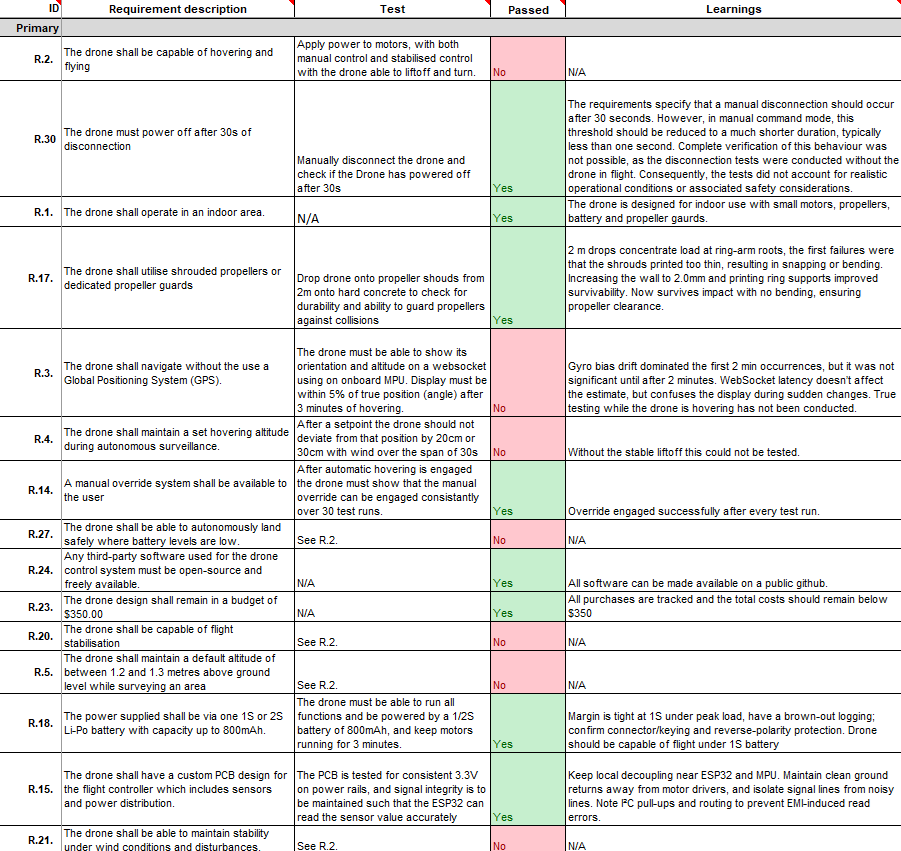
\includegraphics[width=\textwidth]{img/vandv1.png}
\end{figure}

\begin{figure}[H]
    \centering
    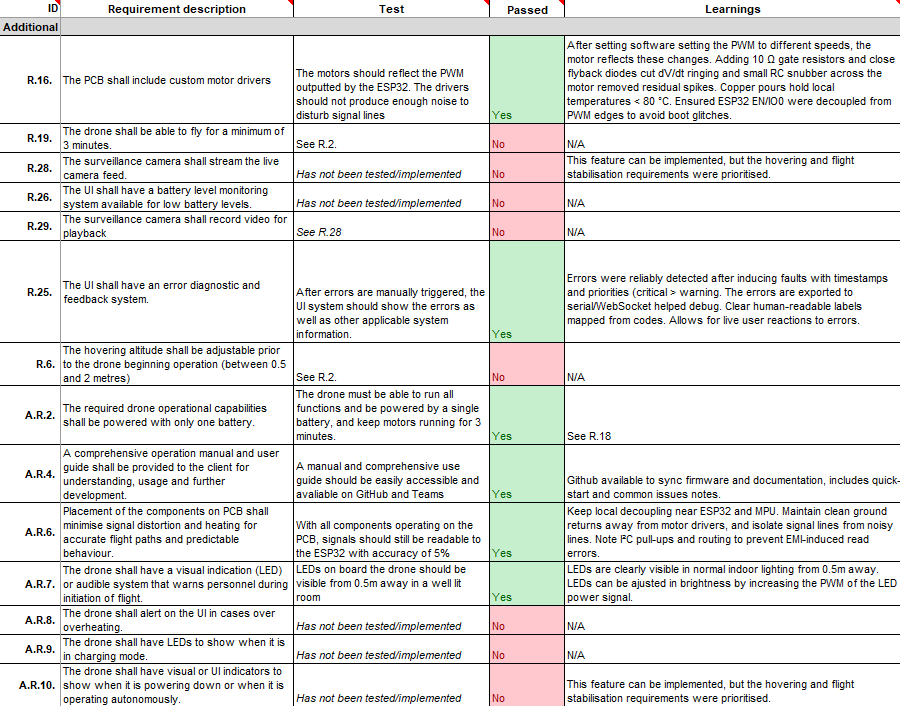
\includegraphics[width=\textwidth]{img/vandv2.png}
\end{figure}

%----------------------------------------------------------%
\pagebreak
\subsection{Hardware Prototypes}
\label{app:pcb-prototypes}

\subsubsection{PCB Prototype 1.0}

\begin{figure}[H]
    \centering
    \begin{subfigure}[b]{0.45\linewidth}
        \centering
        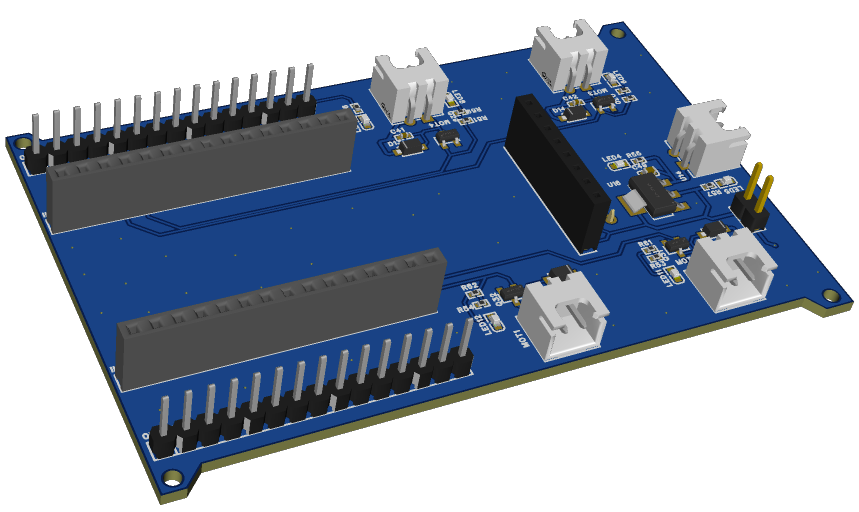
\includegraphics[width=\linewidth]{img/proto-pcb1.png}
        \caption{Overview}
        \label{fig:pcb1-overview}
    \end{subfigure}
    \hfill
    \vfill
    \begin{subfigure}[b]{0.4\linewidth}
        \centering
        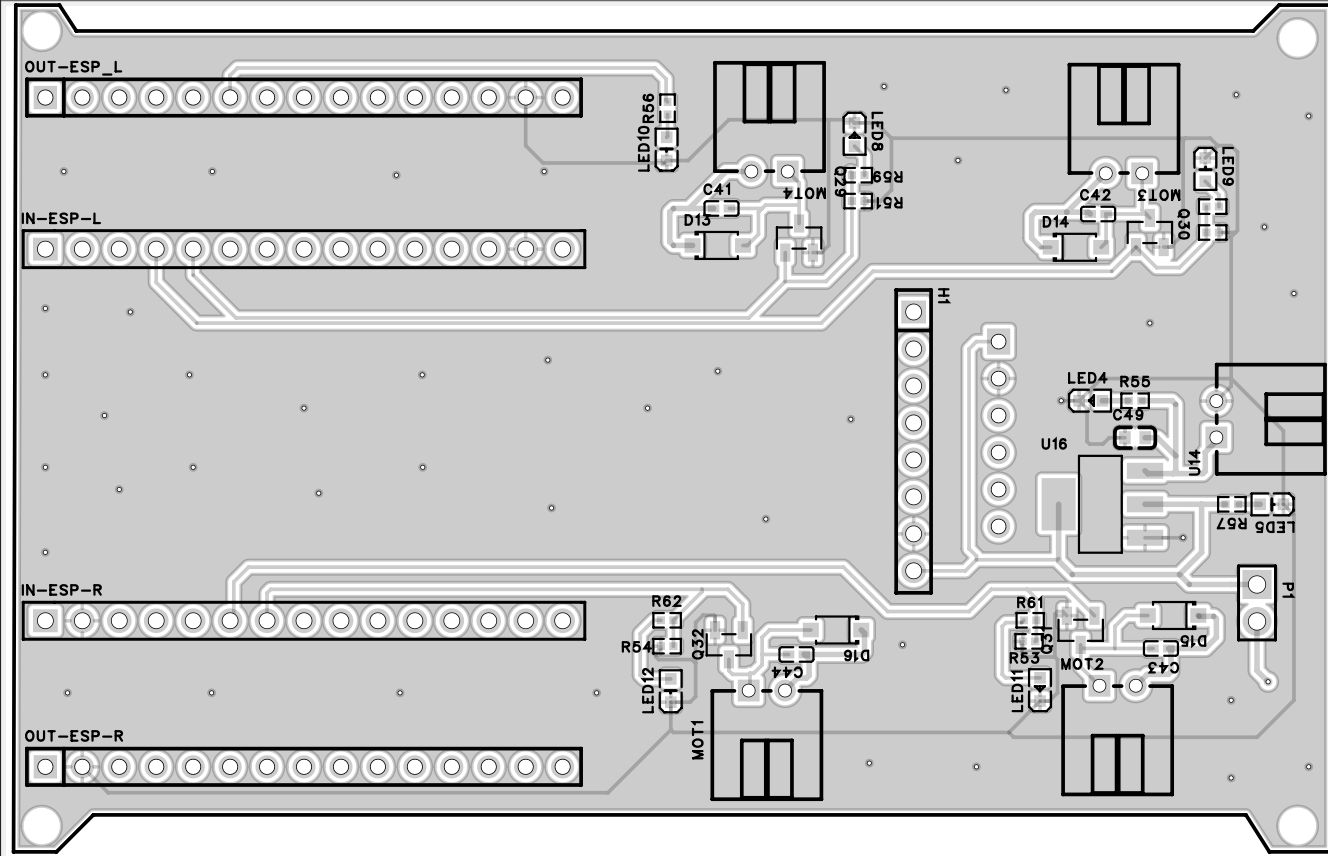
\includegraphics[width=\linewidth]{img/PCBit1_front.png}
        \caption{Front Side}
        \label{fig:pcb1-front}
    \end{subfigure}
    \hfill
    \begin{subfigure}[b]{0.4\linewidth}
        \centering
        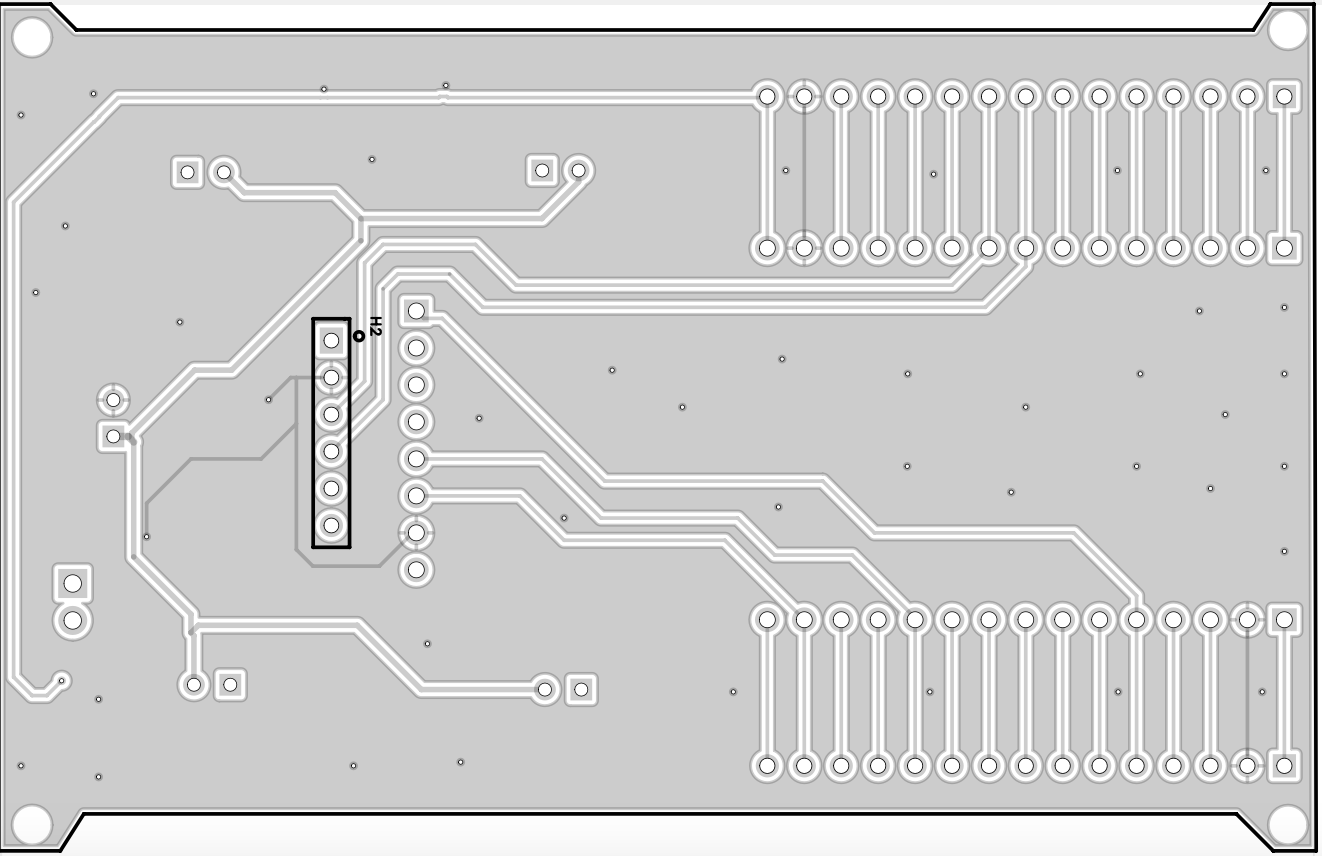
\includegraphics[width=\linewidth]{img/PCBit1_back.png}
        \caption{Back Side}
        \label{fig:pcb1-back}
    \end{subfigure}
    \label{fig:pcb1}
\end{figure}

% \pagebreak
\subsubsection{PCB Prototype 2.0}

\begin{figure}[H]
    \centering
    \begin{subfigure}[b]{0.45\linewidth}
        \centering
        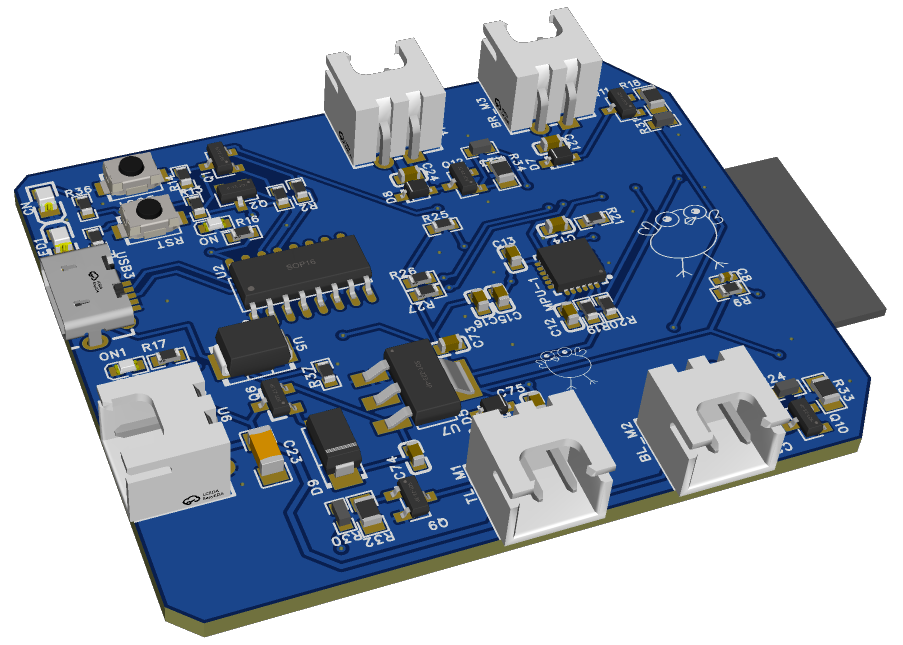
\includegraphics[width=\linewidth]{img/proto-pcb2.png}
        \caption{Overview}
        \label{fig:pcb2-overview}
    \end{subfigure}
    \vfill
    \begin{subfigure}[b]{0.4\linewidth}
        \centering
        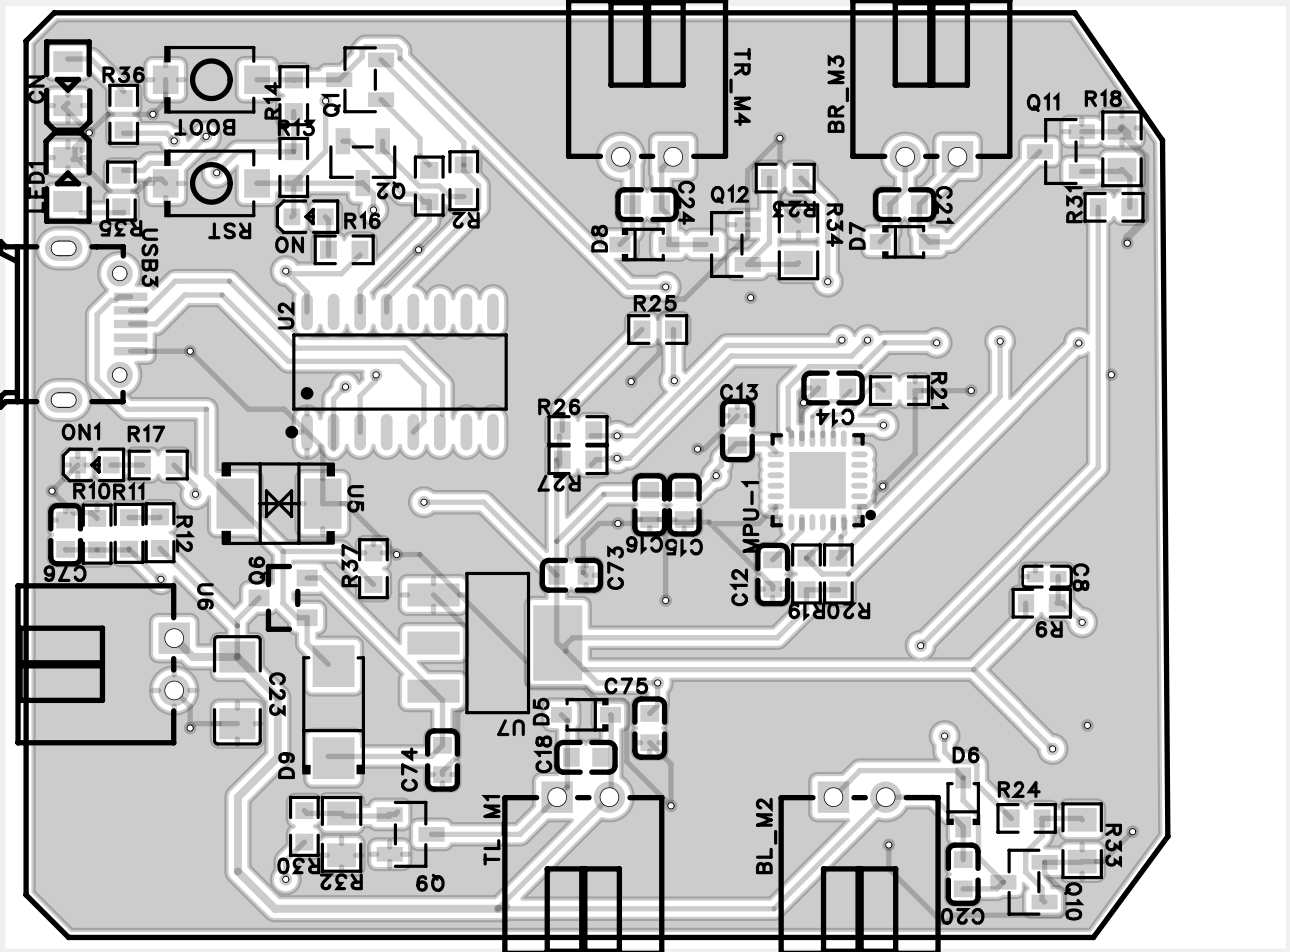
\includegraphics[width=\linewidth]{img/PCBit2_front.png}
        \caption{Front Side}
        \label{fig:pcb2-front}
    \end{subfigure}
    \hfill 
    \begin{subfigure}[b]{0.4\linewidth}
        \centering
        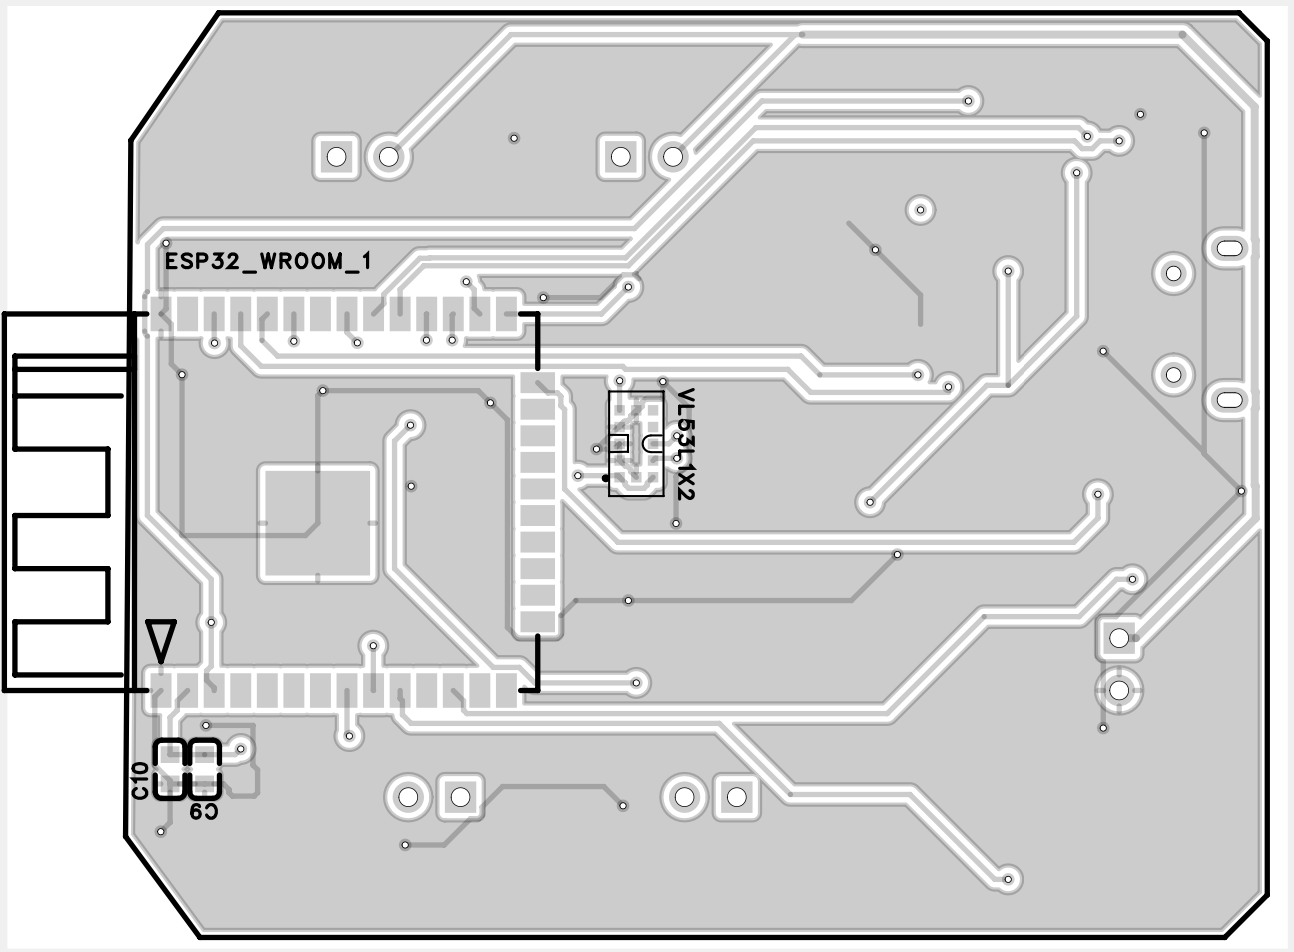
\includegraphics[width=\linewidth]{img/PCBit2_back.png}
        \caption{Back Side}
        \label{fig:pcb2-back}
    \end{subfigure}
    \label{fig:pcb2}
\end{figure}

\pagebreak
\subsubsection{Frame Prototypes}

\begin{figure}[H]
    \centering
    % Prototype 1.0
    \begin{subfigure}[b]{0.48\linewidth}
        \centering
        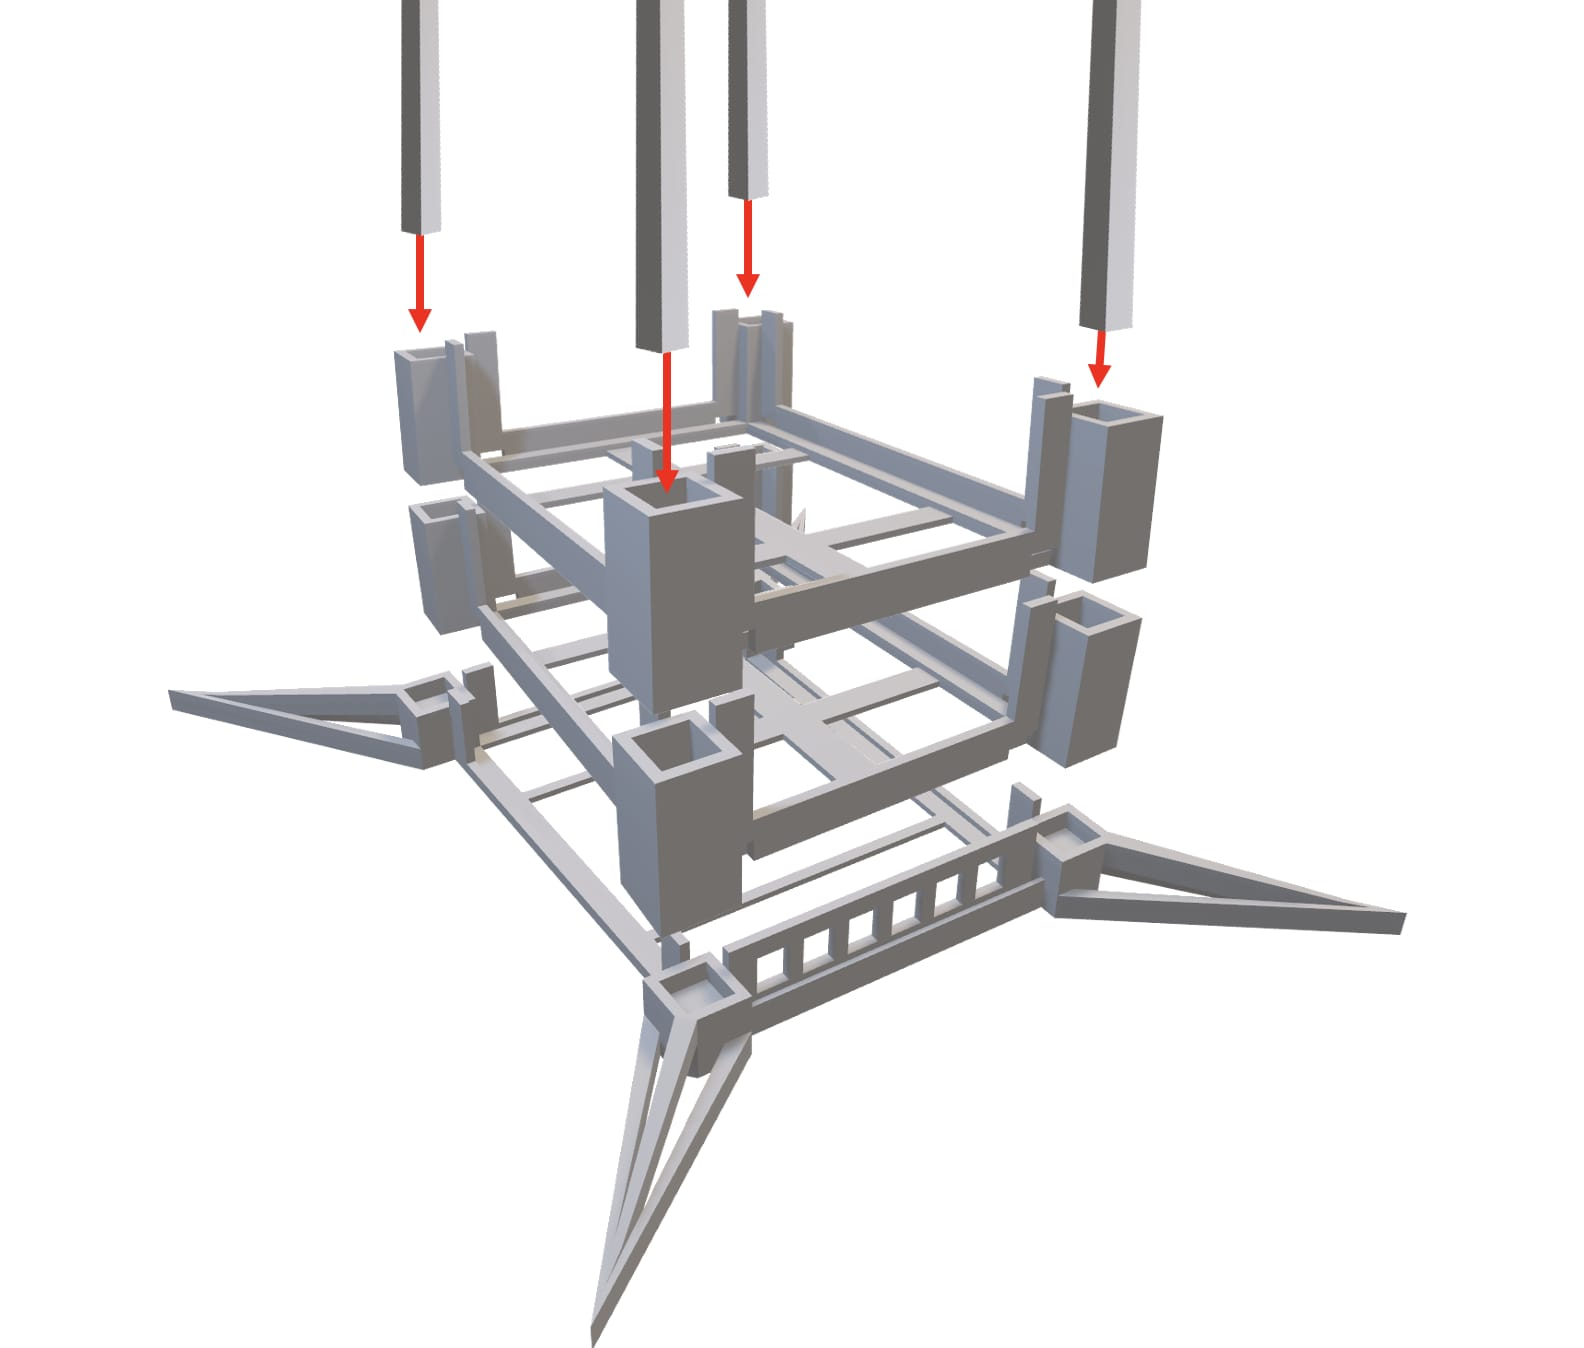
\includegraphics[width=\linewidth]{img/frame-1.PNG}
        \caption{Prototype 1.0}
        \label{fig:frame-proto1}
    \end{subfigure}
    \hfill
    % Prototype 2.0
    \begin{subfigure}[b]{0.48\linewidth}
        \centering
        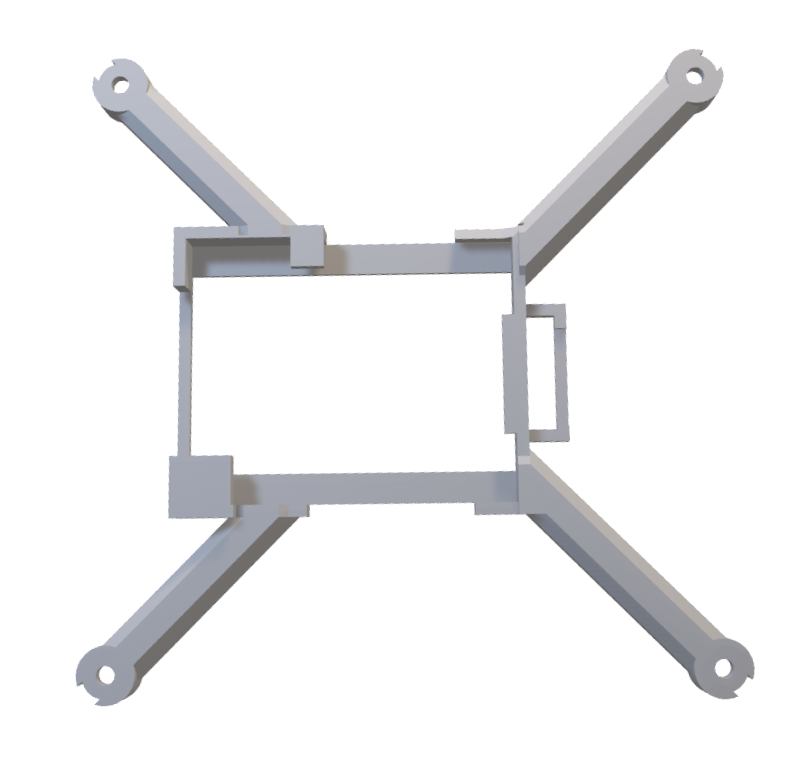
\includegraphics[width=\linewidth]{img/OldFrame.png}
        \caption{Prototype 2.0}
        \label{fig:frame-proto2}
    \end{subfigure}
    \hfill
    % Prototype 3.0 (front)
    \begin{subfigure}[b]{0.48\linewidth}
        \centering
        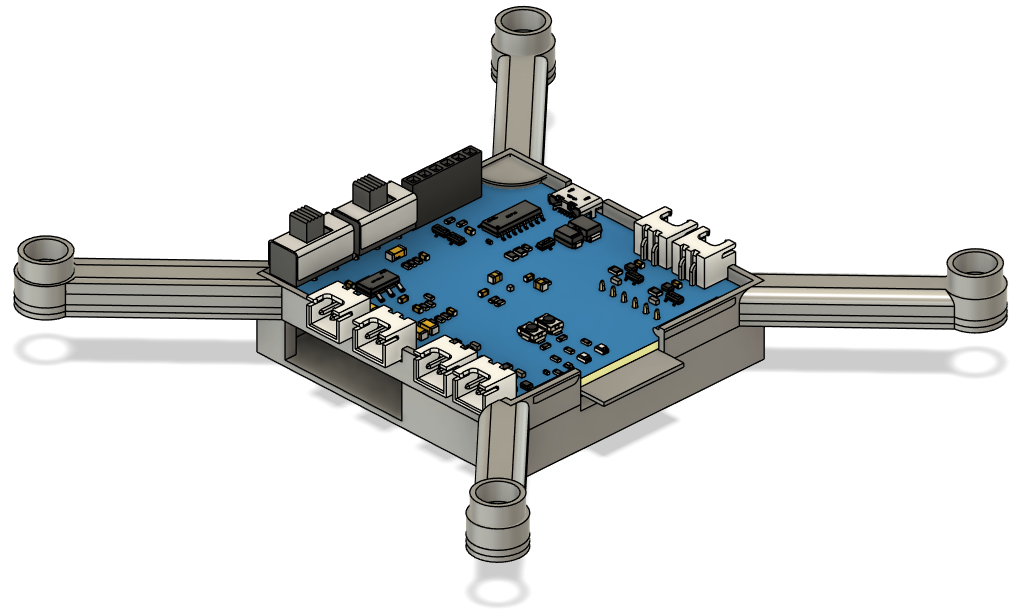
\includegraphics[width=\linewidth]{img/frame-3.png}
        \caption{Prototype 3.0 Front}
        \label{fig:frame-proto3-front}
    \end{subfigure}
    % Prototype 3.0 (back) on a new line
    \vspace{0.3cm}
    \begin{subfigure}[b]{0.48\linewidth}
        \centering
        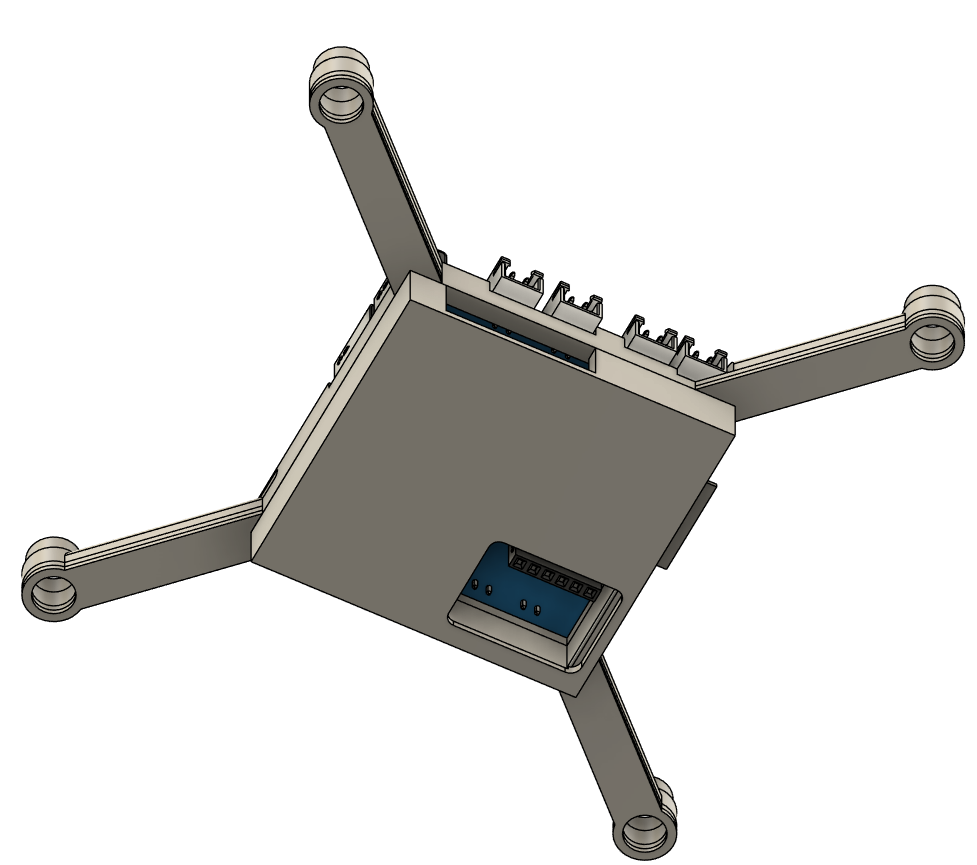
\includegraphics[width=\linewidth]{img/frame-3-back.png}
        \caption{Prototype 3.0 Back}
        \label{fig:frame-proto3-back}
    \end{subfigure}
    % \caption{Development of frame prototypes 1.0 to 3.0, showing front and back views of the final iteration.}
    \label{fig:frame-prototypes}
\end{figure}

\pagebreak
\subsubsection{Assembled Prototype 1.0}

\begin{figure}[H]
    \centering
    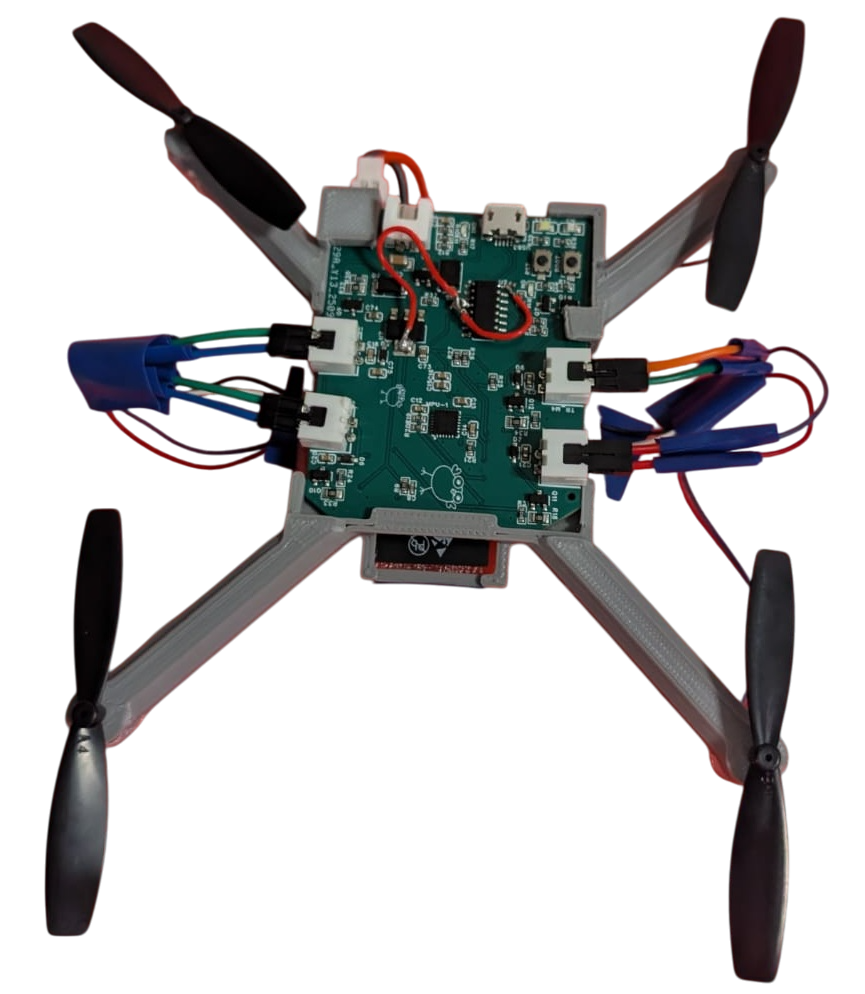
\includegraphics[width=0.55\textwidth]{img/prototype-1-2.png}
\end{figure}

\subsubsection{Assembled Prototype 2.0 For Testing}

\begin{figure}[H]
    \centering
    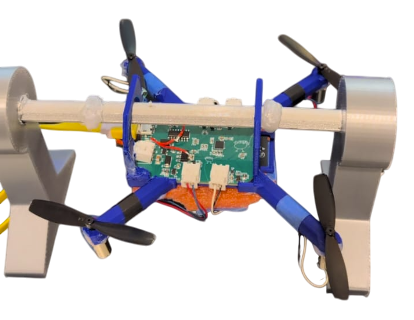
\includegraphics[width=0.7\textwidth]{img/prototype-2.png}
\end{figure}


%----------------------------------------------------------%
\subsection{WebSocket Page}
\label{app:websocket}

\begin{figure}[H]
    \centering
    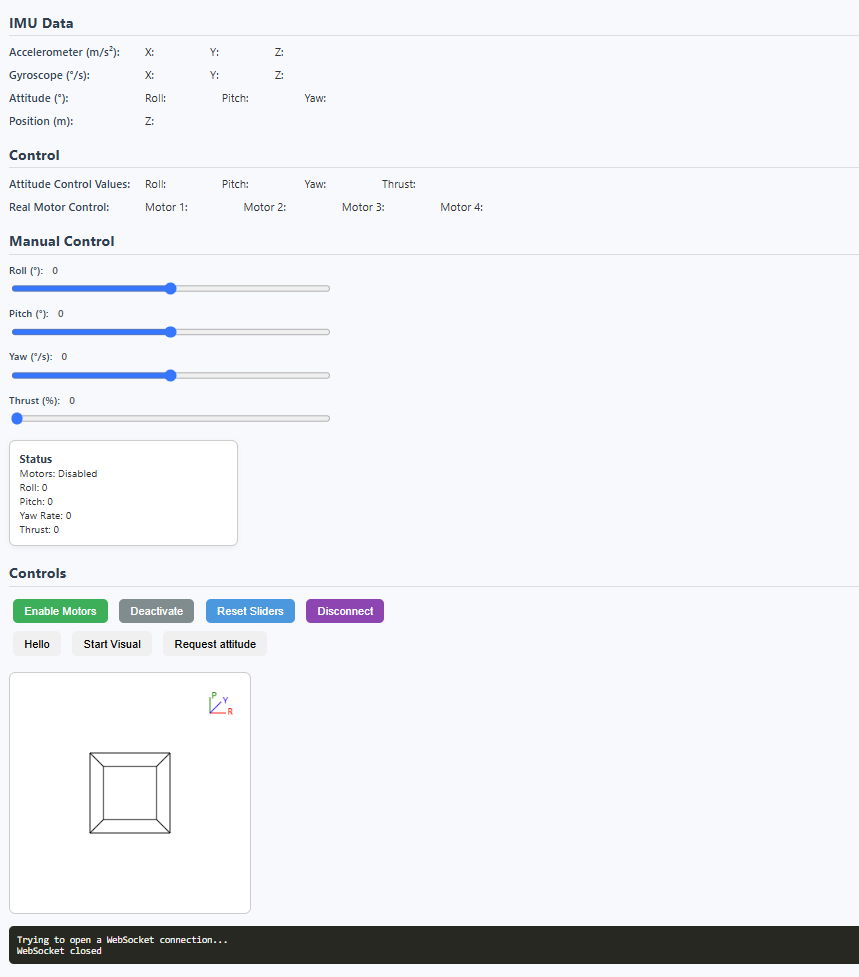
\includegraphics[width=0.98\textwidth]{img/websocket-page.PNG}
    \caption{WebSocket Client Web Page}
\end{figure}

%----------------------------------------------------------%
\pagebreak

\subsection{Stakeholder Engagement}
\label{app:stakeholder-engagement}

\begin{table}[H]
\centering
\caption{Client Meetings, Information Sessions, and Technical Queries - Summary (Weeks 1-5)}
\begin{tabular}{|p{2cm}|p{9.5cm}|p{3cm}|}
\hline
\textbf{Date / Week} & \textbf{Item / Notes} & \textbf{Priority / Additional Notes} \\ \hline
24/07/2025 (W1) & Open-source software must be used. & -- \\ \hline
 & Client requirements may be negotiated with the client. & -- \\ \hline
31/07/2025 (W2) & \textbf{Q1:} Desired action when drone encounters obstacle (stop, reverse, turn around). & Medium \\ \hline
 & \textbf{Client Response:} Stop and hover; shutdown if obstruction persists. Both options desirable. & -- \\ \hline
 & \textbf{Q2:} Requirements for drone movement patterns—preprogrammed or flexible. & High \\ \hline
 & \textbf{Client Response:} Preprogrammed patterns given 1-2 weeks before demo. Custom pattern: simple polygon. & Plan flexible design early \\ \hline
07/08/2025 (W3) & \textbf{Q3:} Two 1S batteries instead of one 2S? Max total capacity 800mAh? & Medium \\ \hline
 & \textbf{Client Response:} Only one battery allowed. Total capacity < 800mAh. & -- \\ \hline
 & Other relevant info: Reaction to wall/obstacles same; automatic obstacle detection and shutdown. & -- \\ \hline
15/08/2025 (W4) & No technical queries this week. & -- \\ \hline
23/08/2025 (W5) & \textbf{Q4:} Mounting IR sensor (VL53L0X) with perpendicular orientation to main PCB. Breakout allowed? & Medium \\ \hline
 & \textbf{Client Response:} Yes. & -- \\ \hline
 & \textbf{Q5:} Can we place coloured/reflective tape for start position? & Low \\ \hline
 & \textbf{Client Response:} Yes. & -- \\ \hline
\end{tabular}
\end{table}

\begin{table}[H]
\centering
\caption{Other Information - Summary (Weeks 1-5)}
\begin{tabular}{|p{2.5cm}|p{12cm}|}
\hline
\textbf{Date / Week} & \textbf{Item / Notes} \\ \hline
24/07/2025 (W1) &
Drifting should be below 10 cm before stabilisation.  \newline 
Object detection is for non-transparent objects only.  \newline 
Surveillance camera must record video and optionally allow hover height adjustment. \newline
Final testing location: MATH151. \newline
ESCs must be part of the PCB. \\ \hline
07/08/2025 (W3) &
No obstacles on ground during demo. \newline
Can use magnetometer and multiple MCU chips, particularly for camera. \newline Camera does not need to be ESP32-based \newline \\ \hline
\end{tabular}
\end{table}

%----------------------------------------------------------%
\pagebreak
\subsection{Requirements Update Summary (Week 6)}
\label{app:req-changes}

\subsubsection{Ranked Requirements - Proposed Changes}

\begin{table}[H]
\centering
\caption{Ranked Requirements Proposed Changes}
\begin{tabular}{|c|c|p{11cm}|}
\hline
\textbf{Rank} & \textbf{No.} & \textbf{Requirement Description} \\ \hline
1 & R.2 & The drone shall be capable of hovering and flying. \\ \hline
2 & R.30 & The drone must power off after 30s of disconnection. \\ \hline
3 & R.1 & The drone shall operate in an indoor area. \\ \hline
4 & R.17 & The drone shall utilise shrouded propellers or dedicated propeller guards. \\ \hline
5 & R.3 & The drone shall navigate without the use of GPS. \\ \hline
6 & R.4 & The drone shall maintain a set hovering altitude during autonomous surveillance. \\ \hline
7 & R.14 & A manual override system shall be available to the user. \\ \hline
8 & R.27 & The drone shall autonomously land safely when battery levels are low. \\ \hline
9 & R.24 & Any third-party software used for the drone control system must be open-source and freely available. \\ \hline
10 & R.7 & \textcolor{red}{\sout{The drone shall be able to navigate autonomously.}} \\ \hline
11 & R.11 & \textcolor{red}{\sout{The drone should be capable of detecting obstacles.}} \\ \hline
12 & R.12 & \textcolor{red}{\sout{The drone shall be capable of avoiding non-transparent obstacles (including walls) by stopping and hovering.}} \\ \hline
13 & R.23 & The drone design shall remain within a budget of \$350.00. \\ \hline
14 & R.20 & The drone shall be capable of flight stabilisation. \\ \hline
15 & R.5 & The drone shall maintain a default altitude of 1.2-1.3 metres above ground level while surveying an area. \\ \hline
16 & R.18 & The power supplied shall be via one 1S or 2S Li-Po battery with a capacity up to 800mAh. \\ \hline
17 & R.15 & The drone shall have a custom PCB design for the flight controller which includes sensors and power distribution. \\ \hline
18 & R.8 & \textcolor{red}{\sout{The drone shall follow a predefined path set before beginning operation.}} \\ \hline
19 & R.13 & \textcolor{red}{\sout{The drone shall power down if it detects an obstacle and the obstacle is not removed within a certain time limit.}} \\ \hline
20 & R.21 & The drone shall maintain stability under wind conditions and disturbances. \\ \hline
\end{tabular}
\end{table}

\begin{table}[H]
\centering
\caption{Ranked Requirements - Final}
\begin{tabular}{|c|c|p{11cm}|}
\hline
\textbf{Rank} & \textbf{No.} & \textbf{Requirement Description} \\ \hline
1 & R.2 & The drone shall be capable of hovering and flying. \\ \hline
2 & R.30 & The drone must power off after 30s of disconnection. \\ \hline
3 & R.1 & The drone shall operate in an indoor area. \\ \hline
4 & R.17 & The drone shall utilise shrouded propellers or dedicated propeller guards. \\ \hline
5 & R.3 & The drone shall navigate without the use of GPS. \\ \hline
6 & R.4 & The drone shall maintain a set hovering altitude during autonomous surveillance. \\ \hline
7 & R.14 & A manual override system shall be available to the user. \\ \hline
8 & R.27 & The drone shall autonomously land safely when battery levels are low. \\ \hline
9 & R.24 & Any third-party software used for the drone control system must be open-source and freely available. \\ \hline
10 & R.23 & The drone design shall remain within a budget of \$350.00. \\ \hline
11 & R.20 & The drone shall be capable of flight stabilisation. \\ \hline
12 & R.5 & The drone shall maintain a default altitude of 1.2-1.3 metres above ground level while surveying an area. \\ \hline
13 & R.18 & The power supplied shall be via one 1S or 2S Li-Po battery with a capacity up to 800mAh. \\ \hline
14 & R.15 & The drone shall have a custom PCB design for the flight controller which includes sensors and power distribution. \\ \hline
15 & R.21 & The drone shall maintain stability under wind conditions and disturbances. \\ \hline
\end{tabular}
\end{table}

\subsubsection{Additional Requirements - Proposed Changes}

\begin{table}[H]
\centering
\caption{Additional Requirements Proposed Changes}
\begin{tabular}{|c|p{11cm}|}
\hline
\textbf{No.} & \textbf{Description} \\ \hline
R.16 & The PCB shall include custom motor drivers. \\ \hline
R.19 & The drone shall be able to fly for a minimum of 3 minutes. \\ \hline
R.28 & The surveillance camera shall stream the live camera feed. \\ \hline
R.9 & \textcolor{red}{\sout{There shall be a predefined set of options for the drone flight.}} \\ \hline
R.26 & The UI shall have a battery level monitoring system available for low battery levels. \\ \hline
R.29 & The surveillance camera shall record video for playback. \\ \hline
R.25 & The UI shall have an error diagnostic and feedback system. \\ \hline
R.6 & The hovering altitude shall be adjustable prior to operation (between 0.5 and 2 metres). \\ \hline
R.10 & \textcolor{red}{\sout{There shall be the option to change the predefined flight pattern to a custom option.}} \\ \hline
A.R.1 & \textcolor{red}{\sout{Pre-defined flight path shall follow a polygonal pattern of fixed altitude.}} \\ \hline
A.R.2 & The required drone operational capabilities shall be powered with only one battery. \\ \hline
A.R.3 & \textcolor{red}{\sout{When an obstacle is detected, the drone shall stop and hover until the obstacle is removed or a timeout occurs.}} \\ \hline
A.R.4 & A comprehensive operation manual and user guide shall be provided to the client. \\ \hline
A.R.5 & \textcolor{red}{\sout{The pre-determined flight path shape shall be adjustable in size.}} \\ \hline
A.R.6 & Placement of PCB components shall minimise signal distortion and heating. \\ \hline
A.R.7 & The drone shall have a visual or audible indication during initiation of flight. \\ \hline
A.R.8 & The drone shall alert on the UI in cases of overheating. \\ \hline
A.R.9 & The drone shall have LEDs to show when it is in charging mode. \\ \hline
A.R.10 & The drone shall have indicators to show when it is powering down or operating autonomously. \\ \hline
\end{tabular}
\end{table}

\subsubsection{Additional Requirements - Final (Post-Change List)}

\begin{table}[H]
\centering
\caption{Additional Requirements - Final}
\begin{tabular}{|c|p{11cm}|}
\hline
\textbf{No.} & \textbf{Description} \\ \hline
R.16 & The PCB shall include custom motor drivers. \\ \hline
R.19 & The drone shall be able to fly for a minimum of 3 minutes. \\ \hline
R.28 & The surveillance camera shall stream the live camera feed. \\ \hline
R.26 & The UI shall have a battery level monitoring system for low battery levels. \\ \hline
R.29 & The surveillance camera shall record video for playback. \\ \hline
R.25 & The UI shall have an error diagnostic and feedback system. \\ \hline
R.6 & The hovering altitude shall be adjustable prior to operation (between 0.5 and 2 metres). \\ \hline
A.R.2 & The required drone operational capabilities shall be powered with only one battery. \\ \hline
A.R.4 & A comprehensive operation manual and user guide shall be provided to the client. \\ \hline
A.R.6 & Placement of PCB components shall minimise signal distortion and heating. \\ \hline
A.R.7 & The drone shall have a visual or audible indication during initiation of flight. \\ \hline
A.R.8 & The drone shall alert on the UI in cases of overheating. \\ \hline
A.R.9 & The drone shall have LEDs to show when it is in charging mode. \\ \hline
A.R.10 & The drone shall have indicators to show when it is powering down or operating autonomously. \\ \hline
\end{tabular}
\end{table}

\textbf{Legend:}  
\textcolor{red}{\sout{Removed}} = Requirement removed in final approved version due to scope or redundancy.

%---------------------------------------------------------%
\pagebreak
\subsection{Code}
\label{app:firmware-code}

%---------------------------------------------------------%
\subsubsection{File Structure}
\begin{figure}[H]
    \centering
    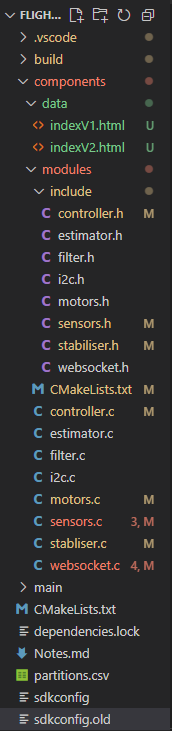
\includegraphics[width=0.2\textwidth]{img/code-files.PNG}
    \caption{File Structure}
\end{figure}

%---------------------------------------------------------%
\subsubsection{sensor.c}

\begin{lstlisting}
//Ref: https://github.com/hibit-dev/mpu6050
//Ref: https://components.espressif.com/components/espressif/mpu6050

#include "i2c.h"
#include "stabiliser.h"
#include "sensors.h"
#include "filter.c"

#define MPU6050_SENSOR_ADDR         0x68
#define MPU6050_WHO_AM_I_REG_ADDR   0x75
#define MPU6050_ACCEL_XOUT_H_ADDR   0x3b 
#define MPU6050_GYRO_XOUT_H_ADDR    0x43
#define MPU6050_PWR_MGMT_1_ADDR     0x6b 
#define MPU6050_GYRO_CONFIG_ADDR    0x1b
#define MPU6050_ACCEL_CONFIG_ADDR   0x1c
#define MPU6050_INT_CFG_ADDR        0x37
#define MPU6050_INT_ENABLE_ADDR     0x38
#define MPU6050_DLPF_ADDR           0x1a
#define MPU6050_H_RESET             0x80
#define MPU6050_SLV4_CTRL_ADDR      0x34
#define MPU6050_MAST_CTRL_ADDR      0x24
#define MPU6050_SMPLRT_DIV_ADDR     0x19

#define GYRO_FULL_SCALE_250_DPS  0x00
#define GYRO_FULL_SCALE_500_DPS  0x08
#define GYRO_FULL_SCALE_1000_DPS 0x10
#define GYRO_FULL_SCALE_2000_DPS 0x18
#define ACC_FULL_SCALE_2G        0x00
#define ACC_FULL_SCALE_4G        0x08
#define ACC_FULL_SCALE_8G        0x10
#define ACC_FULL_SCALE_16G       0x18

#define GYRO_250_SENSITIVITY    (float)((2 * 250.0) / 65536.0)
#define GYRO_500_SENSITIVITY    (float)((2 * 500.0) / 65536.0)
#define GYRO_1000_SENSITIVITY   (float)((2 * 1000.0) / 65536.0)
#define GYRO_2000_SENSITIVITY   (float)((2 * 2000.0) / 65536.0)
#define ACC_2G_SENSITIVITY      (float)((2 * 2) / 65536.0)
#define ACC_4G_SENSITIVITY      (float)((2 * 4) / 65536.0)
#define ACC_8G_SENSITIVITY      (float)((2 * 8) / 65536.0)
#define ACC_16G_SENSITIVITY     (float)((2 * 16) / 65536.0)

#define GYRO_LPF_CUTOFF_FREQ 80
#define ACCE_LPF_CUTOFF_FREQ 30

/* The sensitivity must match the range: */
#define GYRO_SENSITIVITY GYRO_500_SENSITIVITY
#define ACCE_SENSITIVITY ACC_8G_SENSITIVITY
#define GYRO_CONFIG_RANGE GYRO_FULL_SCALE_500_DPS
#define ACCE_CONFIG_RANGE ACC_FULL_SCALE_8G

#define CALIBRATION_SAMPLES 200
#define INT_EN 1
bool use_bias = true;

static const char *TAG = "IMU";

QueueHandle_t acce_queue = NULL;
QueueHandle_t gyro_queue = NULL;
static TaskHandle_t sensor_task_handle = NULL;

static SemaphoreHandle_t mpu6050_data_ready;
static SemaphoreHandle_t sensor_data_ready;

static i2c_master_bus_handle_t bus_handle;
static i2c_master_dev_handle_t dev_handle;
static raw_acce_t raw_acce; 
static raw_gyro_t raw_gyro;
static gyro_t gyro;
static acce_t acce;
static raw_gyro_t gyro_bias = {.x = 0, .y = 0, .z = 0};
static raw_acce_t acce_bias = {.x = 0, .y = 0, .z = 0};
static lpf_data lpf_data_acce[3];
static lpf_data lpf_data_gyro[3];

static bool sensors_init = false;

/* INIT *****************************************************************/
esp_err_t mpu6050_init(i2c_master_bus_handle_t *bus_handle, i2c_master_dev_handle_t *dev_handle) {
    // Intialise the I2C master and device
    i2c_master_init(bus_handle, dev_handle);
    i2c_mpu_device_init(bus_handle, dev_handle);

    ESP_LOGI(TAG, "I2C initialized successfully");
    vTaskDelay(pdMS_TO_TICKS(100)); 
    
    // Reset the registers
    ESP_ERROR_CHECK(mpu6050_register_write_byte(*dev_handle, MPU6050_PWR_MGMT_1_ADDR, MPU6050_H_RESET));
    vTaskDelay(pdMS_TO_TICKS(100)); 
    
    // Set the gyro as the reference
    ESP_ERROR_CHECK(mpu6050_register_write_byte(*dev_handle, MPU6050_PWR_MGMT_1_ADDR, 0x01));

    uint8_t data[2];
    esp_err_t ret = mpu6050_register_read(*dev_handle, MPU6050_WHO_AM_I_REG_ADDR, data, 0x01);
    if (ret != ESP_OK || data[0] != 0x68) return 1;
        
    // Configure the sensor sensitivity
    ESP_ERROR_CHECK(mpu6050_register_write_byte(*dev_handle, MPU6050_ACCEL_CONFIG_ADDR, ACCE_CONFIG_RANGE));
    ESP_ERROR_CHECK(mpu6050_register_write_byte(*dev_handle, MPU6050_GYRO_CONFIG_ADDR, GYRO_CONFIG_RANGE));

    // Enable digital low pass (reduces sample rate from 8kHz to 1kHz)
    ESP_ERROR_CHECK(mpu6050_register_write_byte(*dev_handle, MPU6050_DLPF_ADDR, 0x02)); // 98Hz BW
    ESP_ERROR_CHECK(mpu6050_register_write_byte(*dev_handle, MPU6050_SMPLRT_DIV_ADDR, 0));

    // Enable interrupts
    ESP_ERROR_CHECK(mpu6050_register_write_byte(*dev_handle, MPU6050_INT_ENABLE_ADDR, INT_EN));
    ESP_ERROR_CHECK(mpu6050_register_write_byte(*dev_handle, MPU6050_INT_CFG_ADDR, 0x00));

    // Wake up the IMU
    ESP_ERROR_CHECK(mpu6050_register_write_byte(*dev_handle, MPU6050_PWR_MGMT_1_ADDR, 0x00));
    vTaskDelay(pdMS_TO_TICKS(100)); 

    return ESP_OK;
}

/* De-initialise IMU */
void mpu6050_deinit(i2c_master_bus_handle_t *bus_handle, i2c_master_dev_handle_t *dev_handle) {
    i2c_master_bus_rm_device(*dev_handle);
    i2c_del_master_bus(*bus_handle);
    ESP_LOGI(TAG, "I2C de-initialized successfully");
}

/* MOTION ******************************************************************/
/* Read MPU6050 acceleration */
void mpu6050_read_motion_acce(i2c_master_dev_handle_t *dev_handle, raw_acce_t *raw_acce, acce_t *acce, lpf_data *lpf_data) {
    // Registers (dec):
    // [59-64] Accelerometer

    uint8_t buffer[6];
    esp_err_t ret = mpu6050_register_read(*dev_handle, MPU6050_ACCEL_XOUT_H_ADDR, buffer, sizeof(buffer));

    if (ret != ESP_OK) {
        ESP_LOGE(TAG, "Failed to read from accelerometer");
        return;
    }
    
    raw_acce->x = (((int16_t) buffer[0]) << 8) | buffer[1];
    raw_acce->y = (((int16_t) buffer[2]) << 8) | buffer[3];
    raw_acce->z = (((int16_t) buffer[4]) << 8) | buffer[5];
    
    float x, y, z; 
    x = ((float)(raw_acce->x)) * ACCE_SENSITIVITY;
    y = ((float)(raw_acce->y)) * ACCE_SENSITIVITY;
    z = ((float)(raw_acce->z)) * ACCE_SENSITIVITY;

    acce->x = apply_lpf(&lpf_data[0], x);
    acce->y = apply_lpf(&lpf_data[1], y);
    acce->z = apply_lpf(&lpf_data[2], z);
}

/* Read MPU6050 gyroscope */
void mpu6050_read_motion_gyro(i2c_master_dev_handle_t *dev_handle, raw_gyro_t *raw_gyro, gyro_t *gyro,
                              raw_gyro_t *gyro_bias, lpf_data *lpf_data) {
    // Registers (dec):
    // [67-72] Gyroscope
    uint8_t buffer[6];
    esp_err_t ret = mpu6050_register_read(*dev_handle, MPU6050_GYRO_XOUT_H_ADDR, buffer, sizeof(buffer));
    if (ret != ESP_OK) {
        ESP_LOGE(TAG, "Failed to read from gyro");
        return;
    }

    raw_gyro->x = (((int16_t) buffer[0]) << 8) | buffer[1];
    raw_gyro->y = (((int16_t) buffer[2]) << 8) | buffer[3];
    raw_gyro->z = (((int16_t) buffer[4]) << 8) | buffer[5];
    
    float x, y, z; 
    x = ((float)(raw_gyro->x - gyro_bias->x)) * GYRO_SENSITIVITY;
    y = ((float)(raw_gyro->y - gyro_bias->y)) * GYRO_SENSITIVITY;
    z = ((float)(raw_gyro->z - gyro_bias->z)) * GYRO_SENSITIVITY;

    gyro->x = apply_lpf(&lpf_data[0], x);
    gyro->y = apply_lpf(&lpf_data[1], y);
    gyro->z = apply_lpf(&lpf_data[2], z);
}

void mpu6050_read_motion_raw(i2c_master_dev_handle_t *dev_handle, raw_gyro_t *raw_gyro, raw_acce_t *raw_acce) {
    uint8_t buffer[14];
    mpu6050_register_read(*dev_handle, MPU6050_GYRO_XOUT_H_ADDR, buffer, sizeof(buffer));

    raw_gyro->x = (((int16_t) buffer[0]) << 8) | buffer[1];
    raw_gyro->y = (((int16_t) buffer[2]) << 8) | buffer[3];
    raw_gyro->z = (((int16_t) buffer[4]) << 8) | buffer[5];
    raw_acce->x = (((int16_t) buffer[8]) << 8) | buffer[9];
    raw_acce->y = (((int16_t) buffer[10]) << 8) | buffer[11];
    raw_acce->z = (((int16_t) buffer[12]) << 8) | buffer[13];
}

/* Calibration *************************************************************/
void mpu6050_calibrate(i2c_master_dev_handle_t *dev_handle, raw_gyro_t *raw_gyro, raw_acce_t *raw_acce, raw_gyro_t *gyro_bias, raw_acce_t *acce_bias) {
    uint16_t samples = CALIBRATION_SAMPLES;
    int64_t g_sum_x = 0, g_sum_y = 0, g_sum_z = 0, a_sum_x = 0, a_sum_y = 0, a_sum_z = 0;

    for (int i = 0; i < samples; i++) {
        mpu6050_read_motion_raw(dev_handle, raw_gyro, raw_acce);
        g_sum_x += raw_gyro->x;
        g_sum_y += raw_gyro->y;
        g_sum_z += raw_gyro->z;
        vTaskDelay(pdMS_TO_TICKS(10)); 
    }

    gyro_bias->x = g_sum_x/samples;
    gyro_bias->y = g_sum_y/samples;
    gyro_bias->z = g_sum_z/samples;

    ESP_LOGI(TAG, "Gyro calibrated!");

    ESP_LOGI(TAG, "Gyro Bias: Gx: %.4f Gy: %.4f Gz: %.4f",
        (float)(gyro_bias->x) * GYRO_SENSITIVITY,
        (float)(gyro_bias->y) * GYRO_SENSITIVITY,
        (float)(gyro_bias->z) * GYRO_SENSITIVITY);
}

/**************************************************************/
/* Signal when data is ready from MPU6050 */
void IRAM_ATTR sensorISRHandler(void *arg) {
    // See: FreeRTOS website, xSemaphoreGiveFromISR()
    portBASE_TYPE xHigherPriorityTaskWoken = pdFALSE;
    xSemaphoreGiveFromISR(mpu6050_data_ready, &xHigherPriorityTaskWoken);

    if (xHigherPriorityTaskWoken) {
        portYIELD_FROM_ISR();
    }
}

/* Task *************************************************************/
static void sensor_task(void *arg) {
    // ESP_LOGI(TAG, "Ready to read from mpu6050...");
    while (1) {
        if ((xSemaphoreTake(mpu6050_data_ready, portMAX_DELAY) == pdTRUE)) {
        mpu6050_read_motion_acce(&dev_handle, &raw_acce, &acce, lpf_data_acce);
        xQueueOverwrite(acce_queue, (void *)&acce);

        mpu6050_read_motion_gyro(&dev_handle, &raw_gyro, &gyro, &gyro_bias, lpf_data_gyro);
        xQueueOverwrite(gyro_queue, (void *)&gyro);

        xSemaphoreGive(sensor_data_ready); 
        }
    }
}

void sensor_task_init(void) {
    acce_queue = xQueueCreate(1, sizeof(acce_t));
    gyro_queue = xQueueCreate(1, sizeof(gyro_t));
    mpu6050_data_ready = xSemaphoreCreateBinary();
    sensor_data_ready = xSemaphoreCreateBinary();

    esp_err_t ret = mpu6050_init(&bus_handle, &dev_handle);
    if (ret != ESP_OK) {
        ESP_LOGE(TAG, "Sensor not present or couldn't be read from");
        return;
    }
    vTaskDelay(pdMS_TO_TICKS(100)); 

    if (use_bias) mpu6050_calibrate(&dev_handle, &raw_gyro, &raw_acce, &gyro_bias, &acce_bias);

    for (uint8_t i = 0; i < 3; i++) {
        init_lpf(&lpf_data_acce[i], 1000.0, ACCE_LPF_CUTOFF_FREQ);
        init_lpf(&lpf_data_gyro[i], 1000.0, GYRO_LPF_CUTOFF_FREQ);
    }

    /* Configure interrupt pin */
    gpio_config_t io_conf = {
        .intr_type = GPIO_INTR_POSEDGE, // interrupt of rising edge
        .pin_bit_mask = (1ULL << MPU6050_INT_GPIO_PIN), // bit mask map of the pins for esp
        .mode = GPIO_MODE_INPUT, // set as input mode
        .pull_down_en = 0, // disable pull-down mode
        .pull_up_en = 1, // enable pull-up mode
    };
    
    gpio_config(&io_conf);
    gpio_install_isr_service(0);
    gpio_set_intr_type(MPU6050_INT_GPIO_PIN, GPIO_INTR_POSEDGE);
    gpio_isr_handler_add(MPU6050_INT_GPIO_PIN, sensorISRHandler, (void *)MPU6050_INT_GPIO_PIN);

    ESP_LOGI(TAG, "Sensor interrupt intialised");
    vTaskDelay(pdMS_TO_TICKS(100)); 

    /* Start the task */
    xTaskCreate(sensor_task, "sensor task", 2*1024, NULL, 1, &sensor_task_handle);
    ESP_LOGI(TAG, "Sensor task intialised");
    sensors_init = true; 
}

/**************************************************************/
/* Functions to interface with other tasks */
void waitSensorData() { 
    xSemaphoreTake(sensor_data_ready, portMAX_DELAY);
}

bool sensorsIsInit(void) {
    return sensors_init;
}

void readIMUData(sensor_data_t *sensor_data) {
    xQueuePeek(gyro_queue, (void *)&(sensor_data->gyro), 0);
    xQueuePeek(acce_queue, (void *)&(sensor_data->acce), 0);
}

/**************************************************************/
/* Read from MPU6050 register */
esp_err_t mpu6050_register_read(i2c_master_dev_handle_t dev_handle, uint8_t reg_addr, uint8_t *data, size_t len) {
    return i2c_master_transmit_receive(dev_handle, &reg_addr, 1, data, len, I2C_MASTER_TIMEOUT_MS / portTICK_PERIOD_MS);
}

/* Write to MPU6050 register */
esp_err_t mpu6050_register_write_byte(i2c_master_dev_handle_t dev_handle, uint8_t reg_addr, uint8_t data) {
    uint8_t write_buf[2] = {reg_addr, data};
    return i2c_master_transmit(dev_handle, write_buf, sizeof(write_buf), I2C_MASTER_TIMEOUT_MS / portTICK_PERIOD_MS);
}

/* Initialise MPU device */
void i2c_mpu_device_init(i2c_master_bus_handle_t *bus_handle, i2c_master_dev_handle_t *dev_handle) {
    i2c_device_config_t dev_config = {
        .dev_addr_length = I2C_ADDR_BIT_LEN_7,
        .device_address = MPU6050_SENSOR_ADDR,
        .scl_speed_hz = I2C_MASTER_FREQ_HZ,
    };
    ESP_ERROR_CHECK(i2c_master_bus_add_device(*bus_handle, &dev_config, dev_handle));
}
\end{lstlisting}

%---------------------------------------------------------%
\pagebreak
\subsubsection{filter.c}
\label{app:code-filter}

\begin{lstlisting}
#include "filter.h"
#include <math.h>

/* Initiliase low-pass filter values */
void init_lpf(lpf_data *lpf_data, float fs, float fc) {
    /* Ref: CrazyFlieCore, Filter.c */
    /* Ref: https://www.earlevel.com/main/2003/03/02/the-bilinear-z-transform/ */
    // ohm = tan(pi*Fc/Fs) = K
    // c = K^2 + K/Q + 1, Q = 0.707 (second order butterworth)
    // i.e. 1/Q = 1.414

    float fr = fs/fc; // sampling frequency/cutoff frequency
    float ohm = tanf((float)M_PI/fr);
    float c = 1.0f+2.0f*cosf((float)M_PI/4.0f)*ohm+ohm*ohm; 
    lpf_data->b0 = ohm*ohm/c;
    lpf_data->b1 = 2.0f*lpf_data->b0;
    lpf_data->b2 = lpf_data->b0;
    lpf_data->a1 = 2.0f*(ohm*ohm-1.0f)/c;
    lpf_data->a2 = (1.0f-2.0f*cosf((float)M_PI/4.0f)*ohm+ohm*ohm)/c;
    lpf_data->delayed1 = .0f;
    lpf_data->delayed2 = .0f;
}

/* Apply low-pass filter */
float apply_lpf(lpf_data *lpf_data, float sample) {
    /* Ref: https://en.wikipedia.org/wiki/Digital_biquad_filter */

    //        b0 + b1 z^-1 + b2 z^-2 
    // H(z) = ---------------------- 
    //        1 + a1 z^-1 + a2 z^-2  

    /* Direct form 2 implementation: */
    // w(n) = x(n) - a1 w(n-1) - a2 w(n-2) 
    // y(n) = b0 w(n) + b1 w(n-1) + b3 w(n-2) 
    
    float delayed0 = sample - (lpf_data->delayed1 * lpf_data->a1) - (lpf_data->delayed2 * lpf_data->a2);
    
    if (!isfinite(delayed0)) {
        delayed0 = sample;
    }
        
    float output = (delayed0 * lpf_data->b0) + (lpf_data->delayed1 * lpf_data->b1) + (lpf_data->delayed2 * lpf_data->b2);

    lpf_data->delayed2 = lpf_data->delayed1;
    lpf_data->delayed1 = delayed0;

    return output;
}
\end{lstlisting}
%---------------------------------------------------------%
\pagebreak
\subsubsection{estimator.c}

\begin{lstlisting}
// Ref: CrazyFlieCore, sensorfusion6.c 

#include <math.h>
#include "estimator.h"
#include "sensors.h"
#include "stabiliser.h"

static const char *TAG = "EST";

#define TWO_KP_DEF (2.0f * 0.6f) //(2.0f * 0.4f) // 2 * proportional gain (Kp)
#define TWO_KI_DEF (2.0f * 0.002f) //(2.0f * 0.001f) // 2 * integral gain (Ki)

static const float twoKp = TWO_KP_DEF;    
static const float twoKi = TWO_KI_DEF;    
static float integralFBx = 0.0f;
static float integralFBy = 0.0f;
static float integralFBz = 0.0f;  // integral error terms scaled by Ki


static float grav_x = 0.0f, grav_y = 0.0f, grav_z = 0.0f;
static float qw = 1.0f, qx = 0.0f, qy = 0.0f, qz = 0.0f; 
static float roll = 0.0f, pitch = 0.0f, yaw = 0.0f;
static float velz = 0.0f;

static const float pos_alpha = 0.90f;
static const float vel_alpha = 0.995f;
static const float vel_factor = 1.0f;

static float real_z_acce = 0.0f;
static float base_z = 1.0f; // 1g 
static bool is_acce_calibrated = false;

static bool use_tof = false;

void estimatorComplementary(sensor_data_t *sensor, attitude_t *attitude, float *vel_z, float *pos_z, const uint32_t tick) {
  if (RATE_DO_EXECUTE(ATTITUDE_UPDATE_RATE, tick)) {
    findAttitude(sensor->gyro.x, sensor->gyro.y, sensor->gyro.z, sensor->acce.x, sensor->acce.y, sensor->acce.z, ATTITUDE_UPDATE_DT);
    velocityEstimate(sensor->acce.x, sensor->acce.y, sensor->acce.z, vel_z, ATTITUDE_UPDATE_DT);
    getEulerRPY(attitude); 
  }

  // if (RATE_DO_EXECUTE(ATTITUDE_UPDATE_RATE, tick)) {
  //   positionEstimate(vel_z, pos_z, 0, POS_UPDATE_DT);
  // }
}

/**********************************************************************/
void findAttitude(float gx, float gy, float gz, float ax, float ay, float az, float dt) {
  findQuaterion(gx, gy, gz, ax, ay, az, dt);
  
  // Estimate direction of gravity using quaternion rotation matrix, R(q):
  // [ 1 - 2(qy^2 + qz^2), 2(qx*qy - qw*qz),   2(qx*qz + qw*qy)   ]
  // [ 2(qx*qy + qw*qz),   1 - 2(qx^2 + qz^2), 2(qy*qz - qw*qx)   ]
  // [ 2(qx*qz - qw*qy),   2(qy*qz + qw*qx),   1 - 2(qx^2 + qy^2) ]
  // and point [0, 0, 1].T for gravity (R * p) 
  
  /* Estimate gravity */
  grav_x = 2 * (qx * qz - qw * qy);
  grav_y = 2 * (qw * qx + qy * qz);
  grav_z = qw * qw - qx * qx - qy * qy + qz * qz;

  /* Find gravity from sensors */
  if (!is_acce_calibrated) {
    base_z = (ax * grav_x + ay * grav_y + az * grav_z);
    is_acce_calibrated = true;
  }

  /* Find roll, pitch and yaw */
  if (grav_x>1) grav_x=1;
  if (grav_x<-1) grav_x=-1;

  yaw = atan2f(2*(qx*qy + qw*qz), qw*qw + qx*qx - qy*qy - qz*qz) * 180 / (float)M_PI;

  // These come from rotation matrix for x-axis (Rx) (roll) and rotation matrix for y-axis (Ry) (pitch)
  // Rx(theta) * Ry(psi) * g
  // [     -sin(psi)     ] = -ax => psi = asin(ax)
  // [sin(theta)*cos(psi)] = -ay => cos(psi) = -ay/sin(theta) (1)
  // [cos(psi)*cos(theta)] = -az => from (1): -az = -ay/sin(theta) * cos(theta) -> theta = atan(ay/az)

  pitch = asinf(grav_x) * 180 / (float)M_PI;
  roll = atan2f(grav_y, grav_z) * 180 / (float)M_PI;
}

void velocityEstimate(float ax, float ay, float az, float *vel_z, float dt) {
  real_z_acce = (ax * grav_x + ay * grav_y + az * grav_z) - base_z;
  velz += deadband(real_z_acce, 0.06f) * dt * G;
  velz *= vel_alpha;
  *vel_z = velz;
}

/**********************************************************************/

void positionEstimate(float *vel_z, float *pos_z, float dist, float dt) {
  /* Estimate the position */
  const uint32_t max_sample_age = pdMS_TO_TICKS(50);
  float filtered_z = 0, estimated_z = 0;
  static float prev_estimated_z = 0.0f;

  bool sample_ok = false; // ((xTaskGetTickCount() - tof_data->timestamp) <= max_sample_age);

  if (sample_ok) {
    use_tof = true;
  }

  if (use_tof) {
    filtered_z = (pos_alpha * estimated_z + (1.0f - pos_alpha) * dist);
    estimated_z = filtered_z + (vel_factor * velz * dt);
  } 

  *pos_z = estimated_z;
  *vel_z = (estimated_z - prev_estimated_z) / dt;
  prev_estimated_z = estimated_z;
}

/**********************************************************************/

void getEulerRPY(attitude_t *attitude) {
  attitude->roll = roll; 
  attitude->pitch = pitch;
  attitude->yaw = yaw;
}

void getQuaternion(float *q_w, float *q_x, float *q_y, float *q_z) {
  // Save quaternion 
  *q_w = qw;
  *q_x = qx;
  *q_y = qy;
  *q_z = qz;
}

/**********************************************************************/

void findQuaterion(float gx, float gy, float gz, float ax, float ay, float az, float dt) {
  // gyro: gx, gy, gz
  // acce: ax, ay, az 

  /* Madgwick's implementation of Mayhony's AHRS algorithm (see: http://www.x-io.co.uk/open-source-ahrs-with-x-imu)*/
  // The code is from CrazyFlie

  float recipNorm;
  float halfvx, halfvy, halfvz;
  float halfex, halfey, halfez;
  float qa, qb, qc;

  gx = gx * (float)M_PI / 180 ; // Radians
  gy = gy * (float)M_PI / 180;
  gz = gz * (float)M_PI / 180;

  if(!((ax == 0.0f) && (ay == 0.0f) && (az == 0.0f)))
  {
    // Normalise accelerometer measurement
    recipNorm = invSqrt(ax * ax + ay * ay + az * az);
    ax *= recipNorm;
    ay *= recipNorm;
    az *= recipNorm;

    // Estimated direction of gravity and vector perpendicular to magnetic flux
    halfvx = qx * qz - qw * qy;
    halfvy = qw * qx + qy * qz;
    halfvz = qw * qw - 0.5f + qz * qz;

    // Error is sum of cross product between estimated and measured direction of gravity
    halfex = (ay * halfvz - az * halfvy);
    halfey = (az * halfvx - ax * halfvz);
    halfez = (ax * halfvy - ay * halfvx);

    // Compute and apply integral feedback if enabled
    if(twoKi > 0.0f)
    {
      integralFBx += twoKi * halfex * dt;  // integral error scaled by Ki
      integralFBy += twoKi * halfey * dt;
      integralFBz += twoKi * halfez * dt;
      gx += integralFBx;  // apply integral feedback
      gy += integralFBy;
      gz += integralFBz;
    }
    else
    {
      integralFBx = 0.0f; // prevent integral windup
      integralFBy = 0.0f;
      integralFBz = 0.0f;
    }

    // Apply proportional feedback
    gx += twoKp * halfex;
    gy += twoKp * halfey;
    gz += twoKp * halfez;
  }

  // Integrate rate of change of quaternion
  gx *= (0.5f * dt);   // pre-multiply common factors
  gy *= (0.5f * dt);
  gz *= (0.5f * dt);
  qa = qw;
  qb = qx;
  qc = qy;
  qw += (-qb * gx - qc * gy - qz * gz);
  qx += (qa * gx + qc * gz - qz * gy);
  qy += (qa * gy - qb * gz + qz * gx);
  qz += (qa * gz + qb * gy - qc * gx);

  // Normalise quaternion
  recipNorm = invSqrt(qw * qw + qx * qx + qy * qy + qz * qz);
  qw *= recipNorm;
  qx *= recipNorm;
  qy *= recipNorm;
  qz *= recipNorm;
}

/**********************************************************************/

float invSqrt(float x) {
  return 1.0f/sqrtf(x);
  // float halfx = 0.5f * x;
  // float y = x;
  // long i = *(long*)&y;
  // i = 0x5f3759df - (i>>1);
  // y = *(float*)&i;
  // y = y * (1.5f - (halfx * y * y));
  // return y;
}

float deadband(float value, const float threshold) {
  if (fabsf(value) < threshold)
  {
    value = 0;
  }
  else if (value > 0)
  {
    value -= threshold;
  }
  else if (value < 0)
  {
    value += threshold;
  }
  return value;
}
\end{lstlisting}

%---------------------------------------------------------%
\pagebreak
\subsubsection{controller.c}

\begin{lstlisting}
// Ref: CrazyFlie PID code : ) 

#include "stabiliser.h"
#include "controller.h"
#include "filter.h"
#include "sensors.h"
#include "estimator.h"

static const char *TAG = "PID";
static const bool isManualControl = true;

static attitude_t att_desired = {0};
static attitude_t att_rate_desired = {0};
static attitude_t att_output = {0};
static float actuator_thrust = 0;

PidObject pidRoll;
PidObject pidPitch;
PidObject pidYaw;
PidObject pidRollRate;
PidObject pidPitchRate;
PidObject pidYawRate;
PidObject pidPosX;
PidObject pidPosY;
PidObject pidPosZ;

float thrust_desired = 0; 
float pid_roll = 0, pid_pitch = 0, pid_yaw = 0; 
float pid_is_init = false; 

void controllerInitPID() {
  /* Init all the PID objects */
  pidInit(&pidRollRate, 0, PID_ROLL_RATE_KP, PID_ROLL_RATE_KI, PID_ROLL_RATE_KD,
          ATTITUDE_UPDATE_DT, ATTITUDE_RATE, ATT_RATE_LPF_FC, ATT_RATE_LPF_EN);
  pidInit(&pidPitchRate, 0, PID_PITCH_RATE_KP, PID_PITCH_RATE_KI, PID_PITCH_RATE_KD,
          ATTITUDE_UPDATE_DT, ATTITUDE_RATE, ATT_RATE_LPF_FC, ATT_RATE_LPF_EN);
  pidInit(&pidYawRate, 0, PID_YAW_RATE_KP,   PID_YAW_RATE_KI,   PID_YAW_RATE_KD,
          ATTITUDE_UPDATE_DT, ATTITUDE_RATE, ATT_RATE_LPF_FC, ATT_RATE_LPF_EN);
  
  pidRollRate.int_limit = PID_ROLL_RATE_INT_LIMIT; 
  pidPitchRate.int_limit = PID_PITCH_RATE_INT_LIMIT;
  pidYawRate.int_limit = PID_YAW_RATE_INT_LIMIT;

  pidInit(&pidRoll, 0, PID_ROLL_KP,  PID_ROLL_KI,  PID_ROLL_KD, ATTITUDE_UPDATE_DT,
          ATTITUDE_RATE, ATT_RATE_LPF_FC, ATT_LPF_EN);
  pidInit(&pidPitch, 0, PID_PITCH_KP, PID_PITCH_KI, PID_PITCH_KD, ATTITUDE_UPDATE_DT,
          ATTITUDE_RATE, ATT_RATE_LPF_FC, ATT_LPF_EN);
  pidInit(&pidYaw, 0, PID_YAW_KP,   PID_YAW_KI,   PID_YAW_KD, ATTITUDE_UPDATE_DT,
          ATTITUDE_RATE, ATT_RATE_LPF_FC, ATT_LPF_EN);

  pidRoll.int_limit = PID_ROLL_INT_LIMIT; 
  pidPitch.int_limit = PID_PITCH_INT_LIMIT;
  pidYaw.int_limit = PID_YAW_INT_LIMIT;

  //To-Do: Add position controller

  pid_is_init = true;
}

void controllerPID(sensor_data_t *sensor, state_t *state, setpoint_t *setpoint, control_t *control, const uint32_t tick) {
  if (RATE_DO_EXECUTE(ATTITUDE_RATE, tick)) {
      att_desired.yaw += setpoint->attitudeRate.yaw * ATTITUDE_UPDATE_DT;
      att_desired.yaw = angleLimit(att_desired.yaw); 
  }

  /* Position controller */
  // This gets the thrust from the z velocity (outer-outer loop)
  // To-do: consider x, y tuning
  // (which updates the desired attitude from something other than zero (stable hover))
  // if (RATE_DO_EXECUTE(POSITION_RATE, tick)) {
  //   positionController(&actuator_thrust, &att_desired, setpoint, state);
  // }

  if (RATE_DO_EXECUTE(ATTITUDE_RATE, tick)) {
    actuator_thrust = setpoint->thrust; // Use this for now 
    att_desired.roll = setpoint->attitude.roll;
    att_desired.pitch = setpoint->attitude.pitch; 

    /* Attitude Control */
    /* PID for attitude */
    // This gets the attitude rate from the attitude (outer loop)
    pidRoll.desired = att_desired.roll;
    att_rate_desired.roll = pidUpdate(&pidRoll, state->attitude.roll, true); 

    pidPitch.desired = att_desired.pitch;
    att_rate_desired.pitch = pidUpdate(&pidPitch, state->attitude.pitch, true); 

    float yaw_error;
    yaw_error = setpoint->attitude.yaw - state->attitude.yaw;
    yaw_error = angleLimit(yaw_error);
    pidYaw.error = yaw_error;
    att_rate_desired.yaw = pidUpdate(&pidYaw, state->attitude.yaw, false);
    
    /* Attitude Rate Control */
    // From the attitude rate get an output to the motor! (inner loop)
    pidRollRate.desired = att_rate_desired.roll;
    att_output.roll = pidUpdate(&pidRollRate, sensor->gyro.x, true);
    pidPitchRate.desired = att_rate_desired.pitch;
    att_output.pitch = pidUpdate(&pidPitchRate, sensor->gyro.y, true);
    pidYawRate.desired = att_rate_desired.yaw;
    att_output.yaw = pidUpdate(&pidYawRate, sensor->gyro.z, true);

    control->roll = saturateSignedInt16(att_output.roll);
    control->pitch = saturateSignedInt16(att_output.pitch);
    control->yaw = saturateSignedInt16(att_output.yaw);

    if (isManualControl) {
      control->thrust = scaleThrust(actuator_thrust);
      // control->roll = scaleAngle90(setpoint->attitude.roll);
      // control->pitch = scaleAngle90(setpoint->attitude.pitch); 
      // control->yaw = scaleAngle180(att_desired.yaw); 
    } else {
      control->thrust = actuator_thrust;
    } 

    if (RATE_DO_EXECUTE(LOG_RATE, tick)) {
      ESP_LOGI(TAG, "tick=%lu", (unsigned long)tick);
      ESP_LOGI(TAG, "att_des: [roll=%.2f pitch=%.2f yaw=%.2f] thrust=%.2f",
        att_desired.roll, att_desired.pitch, att_desired.yaw, actuator_thrust);
      ESP_LOGI(TAG, "att_rate_des: [roll=%.2f pitch=%.2f yaw=%.2f]",
       att_rate_desired.roll, att_rate_desired.pitch, att_rate_desired.yaw);
      ESP_LOGI(TAG, "thrust: [act=%.2f out=%.2f]",
      actuator_thrust, control->thrust);
    }
  }
}

/******************************************************************/

void positionController(float *thrust, attitude_t *att_desired, setpoint_t *setpoint, state_t *state) {
  // Not finished
  thrust_desired = setpoint->thrust;

  float cosyaw = cosf(state->attitude.yaw * (float)M_PI / 180.0f);
  float sinyaw = sinf(state->attitude.yaw * (float)M_PI / 180.0f);
  float bodyvx = setpoint->vx;
  float bodyvy = setpoint->vy;
  setpoint->vx = bodyvx * cosyaw - bodyvy * sinyaw;
  setpoint->vy = bodyvy * cosyaw + bodyvx * sinyaw;

  pidPosZ.desired = setpoint->z;
  setpoint->vz = pidUpdate(&pidPosZ, state->z, true);
}

/******************************************************************/

// From CrazyFlie core, PID.C
void pidInit(PidObject* pid, float desired, float kp, float ki, float kd, float dt, float fs, float fc, bool en_filter) {
  pid->desired = desired;
  pid->error = 0;
  pid->prev_error = 0;
  pid->integ = 0;
  pid->deriv = 0;
  pid->kp = kp;
  pid->ki = ki;
  pid->kd = kd;
  pid->int_limit = 5000.0;
  pid->out_limit = 0.0;
  pid->dt = dt;
  pid->d_filter_en = en_filter;

  if (pid->d_filter_en) {
    init_lpf(&pid->d_filter, fs, fc);
  }
}

float pidUpdate(PidObject* pid, float measured, bool update_error) {
  float output = 0.0f;

  if (update_error) {
    pid->error = pid->desired - measured;
  }

  /* Proportional */
  pid->out_p = pid->kp * pid->error;
  output += pid->out_p;

  /* Derivative */
  float deriv = (pid->error - pid->prev_error) / pid->dt;
  if (pid->d_filter_en) {
    pid->deriv = apply_lpf(&pid->d_filter, deriv);
  } else {
    pid->deriv = deriv;
  }

  if (isnan(pid->deriv)) {
    pid->deriv = 0;
  }
  
  pid->out_d = pid->kd * pid->deriv;
  output += pid->out_d;

  /* Integral */
  pid->integ += pid->error * pid->dt;

  // Constrain the integral (unless the int_limit is zero)
  if(pid->int_limit != 0) {
    pid->integ = constrain(pid->integ, -pid->int_limit, pid->int_limit);
  }

  pid->out_i = pid->ki * pid->integ;
  output += pid->out_i;

  // Constrain the total PID output (unless the out_limit is zero)
  if(pid->out_limit != 0) {
    output = constrain(output, -pid->out_limit, pid->out_limit);
  }

  pid->prev_error = pid->error;

  return output;
}

/******************************************************************/
float scaleThrust(float actuator_thrust) {
    // for actuator_thrust between 0-100
    if (actuator_thrust < 0.0f) actuator_thrust = 0.0f;
    if (actuator_thrust > 100.0f) actuator_thrust = 100.0f;
    // Scale 0-100 -> THRUST_MIN-THRUST_MAX
    return (actuator_thrust / 100.0f) * (float)(THRUST_MAX - THRUST_MIN) + THRUST_MIN;
}

float scaleAngle90(float setpoint) {
    return (setpoint/90.0f) * (float)(INT16_MAX);
}

float scaleAngle180(float setpoint) {
    return (setpoint/180.0f) * (float)(INT16_MAX);
}

// Some helpers from CrazyFlie : )
float angleLimit(float angle) {
  float result = angle;

  while (result > 180.0f) {
    result -= 360.0f;
  }

  while (result < -180.0f) {
    result += 360.0f;
  }

  return result;
}

int16_t saturateSignedInt16(float in)
{
  if (in > INT16_MAX)
    return INT16_MAX;
  else if (in < -INT16_MAX)
    return -INT16_MAX;
  else
    return (int16_t)in;
}

float constrain(float value, const float minVal, const float maxVal)
{
  return fminf(maxVal, fmaxf(minVal,value));
}
\end{lstlisting}

%---------------------------------------------------------%
\pagebreak
\subsubsection{stabiliser.c}

\begin{lstlisting}
#include "stabiliser.h"
#include "websocket.h"
#include "sensors.h"
#include "estimator.h"
#include "controller.h"
#include "motors.h"

#define TESTING false
#define YAW_OFF false

static const char *TAG = "STAB";

#define TIMEOUT_STABILIZE pdMS_TO_TICKS(1000)

static TaskHandle_t stabiliser_task_handle = NULL;

static QueueHandle_t socket_data_queue = NULL;
static QueueHandle_t setpoint_queue = NULL;

static uint32_t lastWakeTime;
static const TickType_t xFrequency = 1;

static state_t state = {0};
static setpoint_t setpoint = {0};
static control_t control = {0};
static sensor_data_t sensor_data = {0};
static socket_data_t socket_data = {0};
static tof_data_t tof_data = {0}; //(?)

const static control_t control_reset = {0};

static bool websocket_disconnect = false;

/**************************************************************/

static void stabiliser_task(void* param) {
  uint32_t tick; 

  if (!sensorsIsInit() && !websocket_is_init()) {
    vTaskDelay(portMAX_DELAY);
  }
  ESP_LOGI(TAG, "Ready to fly!");

  lastWakeTime = xTaskGetTickCount(); // not using this right now but may use later
  tick = 1;

  while(1) {
    waitSensorData();
    readIMUData(&sensor_data);
    
    /* Get state estimate */
    // Also position estimate (to-do)
    // wait_for_vlx_data();
    estimatorComplementary(&sensor_data, &state.attitude, &state.vz, &state.z, tick);

    /* Update display data */
    sendDisplaySocket();
    
    /* Get set point */
    getSetpoint(&setpoint); 
    stabiliserLog(tick);

    /* PID controller */
    controllerPID(&sensor_data, &state, &setpoint, &control, tick);

    /******* Testing ********/ 
    control.yaw = 0;
    
    /* Send control points to motors */
    if (setpoint.enable && !websocket_disconnect) {
      powerDistribution(&control); 
    } else {
      powerDistribution(&control_reset); 
    }
    
    // Update tick
    tick++;
    vTaskDelayUntil(&lastWakeTime, xFrequency);
  }
}

bool stabiliserTest(void) {
  bool pass = true;
  pass &= powerDistributionTest(); 
  return pass;
}

/**************************************************************/

void getSetpoint(setpoint_t *setpoint) {
  uint32_t now = xTaskGetTickCount();

  if(xQueuePeek(setpoint_queue, (void *)setpoint, 0) == pdTRUE) {
    // setpoint->attitude.roll = 0;
    // setpoint->attitude.pitch = 0;
    // setpoint->attitudeRate.yaw = 0;

    if (((now - setpoint->timestamp) > TIMEOUT_STABILIZE) && !websocket_disconnect && !TESTING) {
      // To-do: might need to change how the timeout works
      setpoint->enable = false;
      websocket_disconnect = true; 
      ESP_LOGE(TAG, "Websocket timestamp too old, disabling motors");
      return;
    }  
  }

  websocket_disconnect = false; 
}

void setSetpoint(setpoint_t *setpoint) {
  xQueueOverwrite(setpoint_queue, setpoint);
}

void sendDisplaySocket() {
  socket_data.attitude = state.attitude;
  socket_data.z = state.z;
  socket_data.control = control;
  xQueueOverwrite(socket_data_queue, (void *)&socket_data);
}

void readSocketData(sensor_data_t *sensor, socket_data_t *socket_data) {
  xQueuePeek(socket_data_queue, (void *)socket_data, 0);
}

/**************************************************************/

void stabiliserLog(const uint32_t tick) {
  if (RATE_DO_EXECUTE(LOG_RATE, tick)) {
      ESP_LOGI(TAG, "tick=%lu", (unsigned long)tick);
      ESP_LOGI(TAG, "sensor: gyro[%.2f %.2f %.2f] acce[%.2f %.2f %.2f]",
        sensor_data.gyro.x, sensor_data.gyro.y, sensor_data.gyro.z,
        sensor_data.acce.x, sensor_data.acce.y, sensor_data.acce.z);
      ESP_LOGI(TAG, "state: att[roll=%.2f pitch=%.2f yaw=%.2f] vz=%.2f z=%.2f",
        state.attitude.roll, state.attitude.pitch, state.attitude.yaw,
        state.vz, state.z);
      ESP_LOGI(TAG, "setpoint: att[roll=%.2f pitch=%.2f yaw=%.2f] enable %d "
                    "attRate[roll=%.2f pitch=%.2f yaw=%.2f] thrust=%.2f",
        setpoint.attitude.roll, setpoint.attitude.pitch, setpoint.attitude.yaw, setpoint.enable,
        setpoint.attitudeRate.roll, setpoint.attitudeRate.pitch, setpoint.attitudeRate.yaw, setpoint.thrust);
      ESP_LOGI(TAG, "control: roll=%d pitch=%d yaw=%d thrust=%.2f",
        control.roll, control.pitch, control.yaw, control.thrust);
  }
}

void stabiliserTaskInit(void) {
    socket_data_queue = xQueueCreate(1, sizeof(socket_data_t));
    setpoint_queue = xQueueCreate(1, sizeof(setpoint_t));

    /* Init */
    motorsInit();
    PWMTimerInit();
    ESP_LOGI(TAG, "Motor GPIO intialised");

    controllerInitPID();
    ESP_LOGI(TAG, "PID controller intialised");

    /* Tests */
    if (!stabiliserTest()) {
      ESP_LOGE(TAG, "Stabiliser tests failed");
    } else {
      ESP_LOGI(TAG, "Stabiliser tests passed");
    }

    /* Task */
    xTaskCreate(stabiliser_task, "stabiliser task", 3*1024, NULL, 5, &stabiliser_task_handle);
    ESP_LOGI(TAG, "Stabiliser task intialised");
}

\end{lstlisting}

%---------------------------------------------------------%
\pagebreak
\subsubsection{motors.c}

\begin{lstlisting}
// From CrazyFlie core, power_distribution_stock.c
// ESP Driver, motors.c

#include "driver/ledc.h"
#include "motors.h"
#include "stabiliser.h"

static bool isInit = false;
static bool isTimerInit = false;

uint32_t motor_ratios[] = {0, 0, 0, 0};
const uint32_t MOTORS[] = {MOTOR_M1, MOTOR_M2, MOTOR_M3, MOTOR_M4};

static uint32_t idleThrust = DEFAULT_IDLE_THRUST;

static struct {
  uint32_t m1;
  uint32_t m2;
  uint32_t m3;
  uint32_t m4;
} motorPower;

ledc_channel_config_t motors_channel[NBR_OF_MOTORS] = {
    {
        .channel = MOT_PWM_CH1,
        .duty = 0,
        .gpio_num = MOTOR1_GPIO,
        .speed_mode = LEDC_LOW_SPEED_MODE,
        .timer_sel = LEDC_TIMER_0
    },
    {
        .channel = MOT_PWM_CH2,
        .duty = 0,
        .gpio_num = MOTOR2_GPIO,
        .speed_mode = LEDC_LOW_SPEED_MODE,
        .timer_sel = LEDC_TIMER_0
    },
    {
        .channel = MOT_PWM_CH3,
        .duty = 0,
        .gpio_num = MOTOR3_GPIO,
        .speed_mode = LEDC_LOW_SPEED_MODE,
        .timer_sel = LEDC_TIMER_0
    },
    {
        .channel = MOT_PWM_CH4,
        .duty = 0,
        .gpio_num = MOTOR4_GPIO,
        .speed_mode = LEDC_LOW_SPEED_MODE,
        .timer_sel = LEDC_TIMER_0
    },
};

bool powerDistributionTest(void) {
  bool pass = true;
  pass &= motorsTest();
  return pass;
}

void powerDistribution(const control_t *control) {
    int16_t r = control->roll / 2.0f;
    int16_t p = control->pitch / 2.0f;

    motorPower.m1 = limitUint16(control->thrust - r + p + control->yaw);
    motorPower.m2 = limitUint16(control->thrust - r - p - control->yaw);
    motorPower.m3 = limitUint16(control->thrust + r - p + control->yaw);
    motorPower.m4 = limitUint16(control->thrust + r + p - control->yaw);

    // motorPower.m1 = limitUint16(control->thrust);
    // motorPower.m2 = limitUint16(control->thrust);
    // motorPower.m3 = limitUint16(control->thrust);
    // motorPower.m4 = limitUint16(control->thrust);

    if (motorPower.m1 < idleThrust) {
      motorPower.m1 = idleThrust;
    }
    if (motorPower.m2 < idleThrust) {
      motorPower.m2 = idleThrust;
    }
    if (motorPower.m3 < idleThrust) {
      motorPower.m3 = idleThrust;
    }
    if (motorPower.m4 < idleThrust) {
      motorPower.m4 = idleThrust;
    }

    motorsSetRatio(MOTOR_M1, motorPower.m1);
    motorsSetRatio(MOTOR_M2, motorPower.m2);
    motorsSetRatio(MOTOR_M3, motorPower.m3);
    motorsSetRatio(MOTOR_M4, motorPower.m4);
}

/**********************************************************************/

// thrust mapped for 65536 <==> 60 grams
void motorsSetRatio(uint32_t id, uint16_t ithrust) {
    if (isInit) {
        uint16_t ratio;
        ratio = ithrust;
        ledc_set_duty(motors_channel[id].speed_mode, motors_channel[id].channel, (uint32_t)motorsConv16ToBits(ratio));
        ledc_update_duty(motors_channel[id].speed_mode, motors_channel[id].channel);
        motor_ratios[id] = ratio;
    }
}

bool motorsTest(void) {
    int i;
    for (i = 0; i < sizeof(MOTORS) / sizeof(*MOTORS); i++) {
          motorsSetRatio(MOTORS[i], MOTORS_TEST_RATIO);
          vTaskDelay(pdMS_TO_TICKS(MOTORS_TEST_ON_TIME_MS));
          motorsSetRatio(MOTORS[i], 0);
          vTaskDelay(pdMS_TO_TICKS(MOTORS_TEST_DELAY_TIME_MS));
    }
    return isInit;
}

/**********************************************************************/

void motorsInit(void) {
    int i;
    if (isInit) {
        return;
    }
    if (PWMTimerInit() != true) {
        return;
    }
    for (i = 0; i < NBR_OF_MOTORS; i++) {
        ledc_channel_config(&motors_channel[i]);
    }
    isInit = true;
}

void motorsDeInit(void) {
    for (int i = 0; i < NBR_OF_MOTORS; i++) {
        ledc_stop(motors_channel[i].speed_mode, motors_channel[i].channel, 0);
    }
}

bool PWMTimerInit(void) {
    if (isTimerInit) {
        return true;
    }

    ledc_timer_config_t ledc_timer = {
        .duty_resolution = MOTORS_PWM_BITS, // resolution of PWM duty
        .freq_hz = 15000,	// frequency of PWM signal
        .speed_mode = LEDC_LOW_SPEED_MODE, // timer mode
        .timer_num = LEDC_TIMER_0, // timer index
    };

    // Set configuration of timer0 for high speed channels
    if (ledc_timer_config(&ledc_timer) == ESP_OK) {
        isTimerInit = true;
        return true;
    }

    return false;
}

/**********************************************************************/

uint16_t limitUint16(int32_t value) {
  if(value > UINT16_MAX) {
    value = UINT16_MAX;
  } else if(value < 0) {
    value = 0;
  }
  return (uint16_t)value;
}

uint16_t motorsConvBitsTo16(uint16_t bits) {
    return ((bits) << (16 - MOTORS_PWM_BITS));
}

uint16_t motorsConv16ToBits(uint16_t bits) {
    return ((bits) >> (16 - MOTORS_PWM_BITS) & ((1 << MOTORS_PWM_BITS) - 1));
}
\end{lstlisting}

%---------------------------------------------------------%
\pagebreak
\subsubsection{websocket.c}

\begin{lstlisting}

// Ref: ESP-IDF v5.5 "ws_echo_server"
// Ref: https://esp32tutorials.com/esp32-esp-idf-websocket-web-server/

#include "sensors.h"
#include "stabiliser.h"
#include "websocket.h"

static const char *TAG = "WEB";

static httpd_handle_t server = NULL;
static sensor_data_t sensor_data = {0};
static socket_data_t display = {0};
static bool websocket_init = false;

void get_imu_data(char *data, uint8_t len) {
    readIMUData(&sensor_data);
    snprintf(data, len, "imu%06.2f%06.2f%06.2f%06.2f%06.2f%06.2f",
             sensor_data.acce.x, sensor_data.acce.y, sensor_data.acce.z,
             sensor_data.gyro.x, sensor_data.gyro.y, sensor_data.gyro.z);
}

void get_display(char *data, uint8_t len) {
    readSocketData(&sensor_data, &display);
    snprintf(data, len, "rpy%06.2f%06.2f%06.2f%06.2f%06.2f%06.2f%06.2f%06.2f",
             display.attitude.roll, display.attitude.pitch, display.attitude.yaw, display.z,
             (float)display.control.roll, (float)display.control.pitch, (float)display.control.yaw, display.control.thrust);
}

void send_setpoint(char *data, uint8_t len) {
    if (len < sizeof(setpoint_t)) return;
    setpoint_t sp;
    memcpy(&sp, data, sizeof(setpoint_t));
    sp.timestamp = xTaskGetTickCount();
    setSetpoint(&sp);
}

/**************************************************************/

void async_send(void *arg) {
    struct async_send_arg *resp_arg = arg;
    httpd_handle_t hd = resp_arg->hd;
    int fd = resp_arg->fd;

    data_read_function funct = resp_arg->funct; 
    char data[255] = {0};
    funct(data, sizeof(data)-1); // pass the correct data function

    httpd_ws_frame_t ws_pkt;
    memset(&ws_pkt, 0, sizeof(httpd_ws_frame_t));
    ws_pkt.payload = (uint8_t*)data;
    ws_pkt.len = strlen(data);
    ws_pkt.type = HTTPD_WS_TYPE_TEXT;

    httpd_ws_send_frame_async(hd, fd, &ws_pkt);
    free(resp_arg);
}

esp_err_t trigger_async_send(httpd_handle_t handle, httpd_req_t *req, data_read_function funct) {
    struct async_send_arg *resp_arg = malloc(sizeof(struct async_send_arg));
    
    if (resp_arg == NULL) {
        return ESP_ERR_NO_MEM;
    }
    
    resp_arg->hd = req->handle;
    resp_arg->fd = httpd_req_to_sockfd(req);
    resp_arg->funct = funct; 
    esp_err_t ret = httpd_queue_work(handle, async_send, resp_arg);
    
    if (ret != ESP_OK) {
        free(resp_arg);
    }
    
    return ret;
}

/**************************************************************/
/* Handle messages being recieved from clients */
esp_err_t handle_ws_req(httpd_req_t *req)
{
    if (req->method == HTTP_GET) {
        ESP_LOGI(TAG, "Handshake done, the new connection was opened");
        return ESP_OK;
    }

    httpd_ws_frame_t ws_pkt;
    uint8_t *buf = NULL;
    memset(&ws_pkt, 0, sizeof(httpd_ws_frame_t));
    ws_pkt.type = HTTPD_WS_TYPE_TEXT;
    
    // Set max_len = 0 to get the frame len
    esp_err_t ret = httpd_ws_recv_frame(req, &ws_pkt, 0);
    if (ret != ESP_OK) {
        ESP_LOGE(TAG, "httpd_ws_recv_frame failed to get frame len with %d", ret);
        return ret;
    }
    
    // ESP_LOGI(TAG, "frame len is %d", ws_pkt.len);
    if (ws_pkt.len) {
        // ws_pkt.len + 1 is for NULL termination as we are expecting a string 
        buf = calloc(1, ws_pkt.len + 1);
        if (buf == NULL) {
            ESP_LOGE(TAG, "Failed to calloc memory for buf");
            return ESP_ERR_NO_MEM;
        }
        ws_pkt.payload = buf;
        // Set max_len = ws_pkt.len to get the frame payload 
        ret = httpd_ws_recv_frame(req, &ws_pkt, ws_pkt.len);
        if (ret != ESP_OK) {
            ESP_LOGE(TAG, "httpd_ws_recv_frame failed with %d", ret);
            free(buf);
            return ret;
        }
        // ESP_LOGI(TAG, "Got packet with message: %s", ws_pkt.payload);
    }
    // ESP_LOGI(TAG, "Packet type: %d", ws_pkt.type);

    /* Handle messages */
    if (ws_pkt.type == HTTPD_WS_TYPE_TEXT) {
        if (strcmp((char*)ws_pkt.payload, "request imu") == 0) {
            free(buf);
            return trigger_async_send(req->handle, req, get_imu_data);
        } else if (strcmp((char*)ws_pkt.payload, "request rpy") == 0) {
            free(buf);
            ret = trigger_async_send(req->handle, req, get_display);
            return (trigger_async_send(req->handle, req, get_imu_data) || ret); // changes
        }
    }

    if (ws_pkt.type == HTTPD_WS_TYPE_BINARY) {
        if (strncmp((char*)ws_pkt.payload, "set", 3) == 0) {
            // ESP_LOGI(TAG, "Setpoint received");
            if (ws_pkt.len >= 3 + sizeof(setpoint_t)) {
                setpoint_t sp;
                memcpy(&sp, ws_pkt.payload + 3, sizeof(setpoint_t));
                send_setpoint((char*)&sp, sizeof(setpoint_t));
            } 
        }
    }
    
    ret = httpd_ws_send_frame(req, &ws_pkt);
    if (ret != ESP_OK) {
        ESP_LOGE(TAG, "httpd_ws_send_frame failed with %d", ret);
    }
    free(buf);

    return ret;
}

/**************************************************************/

const httpd_uri_t ws = {
        .uri        = "/ws",
        .method     = HTTP_GET,
        .handler    = handle_ws_req,
        .user_ctx   = NULL,
        .is_websocket = true
};

httpd_handle_t start_webserver(void) {
    httpd_handle_t server = NULL;
    httpd_config_t config = HTTPD_DEFAULT_CONFIG();
    
    ESP_LOGI(TAG, "Starting server on port: '%d'", config.server_port);
    if (httpd_start(&server, &config) == ESP_OK) {
        ESP_LOGI(TAG, "Registering URI handlers");
        httpd_register_uri_handler(server, &ws);
        return server;
    }
    ESP_LOGI(TAG, "Error starting server!");
    return NULL;
}

void websocket_task_init(void) {
    ESP_ERROR_CHECK(nvs_flash_init());
    ESP_ERROR_CHECK(esp_netif_init());
    ESP_ERROR_CHECK(esp_event_loop_create_default());
    esp_err_t ret = example_connect();

    if (ret != ESP_OK) {
        ESP_LOGE(TAG, "Server failed to connect");
        return; 
    }

    server = start_webserver();

    websocket_init = true;
}

bool websocket_is_init() {
    return websocket_init;
}
\end{lstlisting}
